% !TeX root = RJwrapper.tex
\title{Package \pkg{wsbackfit} for Smooth Backfitting Estimation of Generalized Structured Models}
\author{by Javier Roca-Pardi\~{n}as, Mar\'{\i}a Xos\'e Rodr\'{\i}guez-\'Alvarez and Stefan Sperlich}

\maketitle

\abstract{% max 150 words
	A package is introduced that provides the weighted smooth backfitting 
	estimator for a large family of popular semiparametric regression models.
	This family is known as {\sl generalized structured models}, comprising, for 
	example, generalized varying coefficient model, generalized additive models, mixtures, potentially including parametric parts. The kernel-based weighted smooth backfitting belongs to the statistically most efficient procedures for this model 
	class. Its asymptotic properties are well-understood thanks to the 
	large body of literature about this estimator. The introduced weights allow for  
    the inclusion of sampling weights, trimming, and efficient estimation under 
    heteroscedasticity. Further options facilitate easy handling of aggregated data, 
    prediction, and the presentation of estimation results. Cross-validation methods are provided which can be used for model and bandwidth selection.\footnote{%
    	The second author acknowledges the support received by the Basque Government through the BERC 2018-2021 program and Elkartek project 3KIA (KK-2020/00049), by the Spanish Ministry of Science, Innovation and Universities through BCAM Severo Ochoa accreditation SEV-2017-0718 and through project MTM2017-82379-R funded by (AEI/FEDER, UE).
    	The third author acknowledges financial support from the
    Swiss National Science Foundation, project 200021-192345.}
    }
%\Keywords{generalized structured models, smooth backfitting, generalized varying coefficient models, generalized additive models, computational statistics.}
%

\section{Introduction and brief review} \label{sec-intro}

The classes of generalized structured models (GSM) of \cite{MN2003}, structured additive regression models \citep{BKL2005}, and semiparametric separable models \citep{RSV2003} are all devoted to harmonizing the fundamental aspects of flexibility, dimensionality and
interpretability \cite[c.f.\ also][]{S1986} for multidimensional regression. In some cases, the particular structure is derived 
from pure theory, sometimes from empirical knowledge, or it is chosen data-adaptively. 
The epithet `structured' underlines the explicit modeling of the structure of a regression 
in order to distinguish it from fully automatic black-box regression or prediction. 
\cite{MN2003} define for response $Y$ with covariate vectors $({\bf Z,X,T,U})$  the GSM class by 
\begin{equation}\label{GSM}
	\Lambda ( Y ) =  G\left\{ {\mathbf Z}, \beta , g({\mathbf X}) \right\} +S\left\{ {\mathbf T},\delta ,s ({\mathbf U})\right\} \epsilon = G\left\{ {\mathbf Z}, \beta , g({\mathbf X}) \right\} +\varepsilon \ ,
\end{equation}
with $\Lambda$, $G$, $S$ parametric known functions, $\beta $, $\delta $ unknown 
finite-dimensional parameter, $g (\cdot )$, $s (\cdot)$ unknown nonparametric functions, and $\epsilon, \varepsilon$ fulfilling \( E[\epsilon | {\mathbf Z},{\mathbf X} ]=E[\varepsilon | {\mathbf Z},{\mathbf X} ]=0 \). While $\Lambda$ is a transformation with potentially unknown parts which can be estimated along \cite{LSVK2008}, $G$ and $S$ are link functions that also determine further structures. For instance, for a partial linear varying coefficient model \citep{PMLL2015} with ${\mathbf Z}=(Z_1,\cdots ,Z_d,{\mathbf Z}_\kappa)$, ${\mathbf X}=(X_1,\cdot ,X_d)$, where $Z_1$ to $Z_d$ and $X_1$ to $X_d$ are scalars, and ${\mathbf Z}_\kappa$ a vector of the length of $\beta$, function $G$ defines 
\begin{equation}\label{VCM}
	G\left\{ {\mathbf Z}, \beta , g ({\mathbf X}) \right\} = 
	\underline{G}\left\{ \eta ({\mathbf Z},\beta , g({\mathbf X})) \right\} = \underline{G}\left\{ g_0+\sum_{j=1}^{d}
	g_j(X_j )Z_{j} + {\mathbf Z}_\kappa^t\beta \right\} \ ,
\end{equation}
with index $\eta$ and a known link function $\underline{G}$.
You may also allow that some, or all of the $X_j$, $j=1,\ldots ,d$ are identical; 
the same holds for the $Z_j$, etc. Moreover, by setting $Z_j\equiv 1$ $\forall j$ 
with all $X_j$ being different, you obtain the generalized additive model (GAM).
A detailed discussion on identifiability is provided in \cite{LMP2012}.

Since \cite{HT1990} introduced their backfitting algorithm, additive models have become quite popular in statistics, particularly in biometrics, technometrics, and environmetrics. \cite{OR1997} and \cite{O2000} derived asymptotic theory for that classical backfitting estimator with kernel smoothing. \cite{MLN1999} developed asymptotic theory for a modified version, the smooth backfitting (SB) estimator, under weaker assumptions on the data like the allowance for strong correlation of the covariates. \cite{MN2003} extended this method to the general GSM class (\ref{GSM}), and \cite{RS2010} proposed a common algorithm for it. Many extensions have been developed, procedures for bandwidth selection \cite[e.g.,][]{MP2005}, quantile regression \citep{LMP2010}, and further asymptotic theory for particular cases \cite[see e.g.,][for GAM]{YPM2008}. Most recent contributions extend SB to additive inverse regression \citep{BDHB2016}, proportional hazards \citep{HMMMN2017}, or regression with error-in-variables \citep{HP2018}. All SB procedures and their theory are kernel-based. 

The main advantage of SB is, apart from its excellent numerical performance proven by \citet{NS2005} and \cite{RS2010}, compared to the classical backfitting, that there exists a comprehensive literature that studies its statistical behavior and underlying assumptions. It provides the exact and complete asymptotic theory of SB, such that today this estimator is well understood. The only drawback has been that so far, there  hardly existed an easily available software for this estimator, except the R-package \CRANpkg{sBF} of \cite{RPsBF} for the basic additive model. But due to its complexity, practitioners typically abstain from implementing it themselves. Therefore, the \CRANpkg{wsbackfit} R-package has been developed which provides the weighted SB for all models listed in the next section, including a data-driven bandwidth selector. The package is freely available from the Comprehensive R Archive Network (CRAN) at \url{ https://CRAN.R-project.org/package=wsbackfit} \citep{R20}. Thus, this package closes the gap between the huge
body of existing and still increasing literature about SB on the one side, and its potential use on the other, providing the necessary software.   
We  hope it is soon extended by procedures for the various, partly above cited, extensions. 


It is to be mentioned that there certainly exist R packages for alternative methods to estimate related models. Before briefly discussing some of the most advanced packages, let us mention the reviews of \cite{BT2008}, which reviewed spline-based methods, and \cite{FKL2004} which reviewed (spline-based) Bayesian methods. 

Maybe the broadest set of models can be handled by the package \CRANpkg{BayesX} \citep{RPBayesX}. It embraces several well-known regression models such as GAM, generalized additive mixed models (GAMM), generalized geo-additive mixed models (GGAMM), dynamic models, varying coefficient models (VCM), and geographically weighted regression. Besides exponential family regression, \pkg{BayesX} also supports non-standard regression situations such as regression for categorical responses, hazard regression for continuous survival times, and continuous-time multi-state models; see also its support platform \url{http://www.uni-goettingen.de/de/bayesx}. It has been created by \citet{BKL2005} and \citet{KBBL2008}.

The R package \CRANpkg{gam} \citep{RGam} presents considerable enhancements of the S-PLUS version going back to \citet{HT1990}. It uses classical backfitting to combine different smoothing or fitting methods, particularly local regression and smoothing splines. Another powerful package is \CRANpkg{mgcv} \citep{W2017}, which allows the fitting of generalized additive (mixed) models, with smoothing parameter estimation done by (restricted) marginal likelihood or generalized cross-validation, 
and uses iterated nested Laplace approximation for fully Bayesian inference.
%The {\bf VGAM} package of \citet{Y2010} tried to extend {\bf gam} for fitting vector generalized linear and additive models. It is based on an iteratively re-weighted least squares algorithm and pretends to allow for over-dispersion parameter that depend on covariates. In practice it shows several numerical problems; for example, it always failed when we tried to use it with a negative binomial or similar distributions. 
Another powerful and well-functioning package is \CRANpkg{GAMLSS} of \citet{SR2007}. It is based on penalized likelihood estimation combined with classical backfitting. While \pkg{mgcv} models the index function, \pkg{GAMLSS} models the location, scale, and shape functions by additive linear mixed models. 
It has been created to tackle many interesting distributions of $Y$.  When speaking of likelihood based approaches, one should also mention a method introduced by \citet{TB2006}. Their R-package \CRANpkg{GAMBoost} can be used to fit a GAM by likelihood based boosting, suited for a large number of predictors.

Regarding kernel-based methods that consider related or specific cases of (\ref{GSM}), there are, for example, marginal integration \citep{LN1995} for additive interaction models \citep{STY2002}, and local polynomials for smooth varying coefficients \citep{LR2010}. The latter is implemented in the \CRANpkg{np} package \citep{HR2008}, and turned out to be very competitive when compared to the before-mentioned spline-based packages \citep{ST2015}.


\section{The models that can be estimated by wsbackfit} \label{sec-models}

The aim is to estimate a GSM as introduced in (\ref{GSM}). In the moment of estimation, one has to be specific about $\Lambda$, $G$, and $S$. We concentrate on the popular cases, in particular on those that maintain additivity or a similar separability structure. This way, the estimates provide an easy interpretation, and overcome the curse of dimensionality, which else is inherited by more complex models. To the best of our knowledge, all existing smooth backfitting methods follow the suggestion of \cite{MN2003} to estimate the mean and variance part subsequently, say, first $G\{ \cdots \}$, then $S\{ \cdots \}$. Our implementation follows the suggestion of \cite{RS2010} to allow for 
a (re-)estimation of the mean part ($G\{ \cdots \}$) including weights obtained from the estimation of the variance part ($S\{ \cdots \}$) to potentially increase the efficiency. 
Note, however, that in nonparametrics, it is often not clear to what extent an efficiency gain can be achieved this way; see for example the discussion in \cite{XiaoEtal2003}.
All proposed methods we are aware of, are two- or three-step procedures
similar to what we propose here. 
The estimation of the variance part is performed in the second step by regressing the squared residuals on $({\bf T,U})$, using the same procedure as for $G\{ \cdots \}$. Therefore it is sufficient to concentrate in the following on the mean regression, which can equally well be applied to squared residuals for estimating $S\{ \cdots \}$.

As said, the SB idea for GSM, together with some general results about its asymptotic behavior, was introduced by \cite{MN2003}; specific algorithms and their implementation were introduced and studied in \citet{RS2010}. Detailed information about the implementation is given in a technical report \citep{RS2008}. The implemented algorithms in \pkg{wsbackfit} are modified versions to speed up the procedure by binning techniques and a combination of parametric linear with local constant kernel regression; see below. The models considered in this package are semiparametric in the sense that they contain parametric as well as nonparametric components. Most of them could be seen as extensions of a generalized linear model (GLM) of type $G({\mathbf Z},\beta ,g({\mathbf X})) = \underline{G} \big(\eta ({\mathbf Z},\beta,g({\mathbf X})) \big) = \underline{G} ( g_0 + \alpha^t {\mathbf X}+ \beta^t {\mathbf Z}  )$, see for example \cite{MN1989}. So far, this package does not tackle random effects.

Regarding the choice of $G$, you have first to decide about the link $\underline{G}$. For each conditional distribution, there exists a canonical one: for the conditional Gaussian distribution, this is the identity. 
For a binary response, it is the Logit $({1+1/exp( \bullet )})^{-1}$, and for a
conditional Poisson it is $exp(\bullet )$. Note that the latter can also be used for Pseudo-Poisson estimation. The choice of $\underline{G}$ is certainly linked to the specification of $\Lambda$ which is supposed to be known. Then, such transformation of $Y$ can be performed a priori by the practitioner. Therefore, we henceforth suppress $\Lambda$, to simplify our notation. For $\Lambda$ entailing unknown parameters, consult \cite{LSVK2008}.
	
\citet{RS2010} showed that the estimation procedure for all these models can be summarized in one common feasible minimization problem, namely
\begin{equation} \label{proj-ideaW}
minimize \;\; \int \sum_{i=1}^n \left[ \tilde Y_i - \eta \{{\mathbf Z}_i ,\beta ,g({\mathbf x}) \} \right]^2 W_i \cdot K_h ({{\mathbf x}-{\mathbf X}_i}) \ d{\bf x} \ ,
\end{equation}
where $\tilde Y_i$ is the transformed (e.g.\ by $\Lambda$) 
or linearized (in local scoring if the link is not the identity) response $Y_i$, and $W_i$ is a weight. For example, in the generalized additive model with $\beta = 0$ we have covariates $Z_j \equiv 1$ for $j=1,\ldots, d$, $W_i$ contains the local scoring weights with $\tilde Y_i$ being the accordingly adjusted dependent variable. Further, $K_h(v) = h^{-1} K(v/h)$ with $K(\cdot )$ is the kernel function. It is well known that asymptotically, the choice of smoothing kernel does not have an important impact, as to a large part the kernel effect is compensated by an adequate bandwidth choice. We allow the user to choose between the Epanechnikov kernel which is asymptotically the most efficient one, and the Gaussian kernel which is popular as it helps to avoid some of the numerical problems that may arise in areas where data are sparse.

We call our procedure `weighted smooth backfitting' to emphasize that the user has the option to include a vector of additional weights. % as suggested by \citet{RS2010}. 
As said, by putting the usual kernel weights apart,
part of the weighting comes from local scoring in order to account for the link function
$\underline{G}$.\footnote{%
    \citet{YPM2008} propose a somewhat different algorithm for GAMs replacing local scoring by an alternative that makes asymptotic theory simpler.} 
However, independently from the link function, the practitioner might also want to include sampling weights, e.g., when using administrative data, or trimming weights, e.g., for excluding boundary points. A particular case is when additional weights are included to improve the efficiency of your estimators, e.g., to account for the (co-)variance structure.   \citet{RS2010} estimated in a first step the mean function, afterward the variance from the squared residuals, and used these in the third step as additional weights when re-estimating the conditional mean. The resulting average mean squared error was substantially smaller than the one of the original estimator, which ignored the (co-)variance structure; recall our discussion at the beginning of this section. 

The models that package \pkg{wsbackfit} can presently estimate are: 
a partial linear GAM, a generalized partial linear varying coefficient 
model (GVCM), and combinations of them. The first one is a generalization of a GLM by replacing some linear components with additive nonparametric functions, 
\begin{equation*} \label{eq3}
E \left[ {Y\vert {\bf X},{\bf Z}} \right] = \underline{G} \left( {g_0 + \sum\nolimits_{j = 1}^d g_j \left( {X_j } \right) + \beta^t {\mathbf Z} } \right) \ ,
\end{equation*}
where  $X_1$ to $X_d$ are scalars, and ${\mathbf Z}$ is the vector of all covariates that are supposed to enter the index function $\eta$ linearly. The $g_j $ are nonparametric functions.\footnote{%
	For identification we follow \cite{LMP2012}, and \cite{RS2010} for implementation with  modifications like the inclusion of a parametric linear slope for each $g_j$, see below.}
It is actually true that this is a special case of the partial linear GVCM of the form (\ref{VCM}), obtained by setting $Z_1=Z_2=\cdots =Z_d=1$. We list them nonetheless separately because, besides the slightly different implementation, we want the reader to recognize the difference in the modeling approach.     
First, the GVCM is a generalization of a GLM in ${\mathbf Z}$, as could be seen in (\ref{VCM}).  
And second, here we allow for all the flexibility suggested by \cite{LMP2012} regarding the alterations of covariates $X_j$ and $Z_j$.
For example, all $X_1,\ldots ,X_{d_1}$ with $d_1\le d$ 
could be the same scalar variable $X_1$ such that  
\begin{equation} \label{eq51}
\sum\nolimits_{j = 1}^{d_1} g_j \left( {X_j } \right) Z_j  =
\sum\nolimits_{j = 1}^{d_1} \big\{ g_{j0} + g_{j1} \left( {X_1 } \right) \big\} Z_j   \ ,
\end{equation}
with $g_{j0}$ unknown constants and $g_{j1}$ unknown nonparametric functions;
or, alternatively, all $Z_1,\ldots ,Z_{d_1}$ with $d_1\le d$ 
could be the same scalar variable $Z_1$ such that  (with $g_{10}$ still a constant)
\begin{equation} \label{eq52}
\sum\nolimits_{j = 1}^{d_1} g_j \left( {X_j } \right) Z_j  =
\big\{ g_{10} + \sum\nolimits_{j = 1}^{d_1} g_{j1} \left( {X_j } \right) \big\} Z_1   \ .
\end{equation}
Certainly, you can have a mixture of both, as long as the identification conditions of \cite{LMP2012} are fulfilled to guarantee that the model does not suffer from concurvity. This includes the possibility that some variables appear in both sets, ${\bf {X}}$ and ${\mathbf Z}$. This could be of particular interest when defining different types of interactions. 

Finally, one can include all together, i.e., nonparametric additive terms, nonparametric varying coefficients, and a parametric (linear) part like  
\begin{equation} \label{eq6}
E \left[ {Y\vert {\bf {X,Z}}} \right] = \underline{G} \left\{  {g_0 + \sum\nolimits_{j = 1}^{d_1} g_j \left( {X_j } \right) Z_j + \sum\nolimits_{j = d_1+1}^{d} g_j \left( {X_j } \right) + \beta^t {\mathbf Z}_\kappa } \right\} \ ,
\end{equation}
with ${\bf X}$ as before, ${\bf Z}=(Z_1,\ldots ,Z_{d_1},{\mathbf Z}_\kappa)$ a set of scalar variables $Z_1,\ldots ,Z_{d_1}$, and a vector ${\mathbf Z}_\kappa$.
Again, some of the $X_j$ may represent the same variable; the same holds for the $Z_j$, $j=1,...,d$.


\section{Cross-validation, bandwidths, and computational issues} \label{sec-banda}

Cross-validation (CV) can be used for model selection in general.
However, for the sake of presentation we describe here
our implementation in the context of bandwidth selection.
 

\subsection{Cross-validation for bandwidth}

All nonparametric estimates of the $ g_j (X_j)$ in (\ref{eq6}) depend on some bandwidths $h_1,\ldots,h_d$, which can be preset by the user. Alternatively, the package provides the option to choose the bandwidths data-adaptively via CV. Our implementation even allows for a mixture of both, i.e., users can fix some bandwidths and choose the others by CV. 
Albeit we use binning techniques, performing CV can render the program pretty slow, especially for high dimensions and huge data sets. Generally, our implementation follows the ideas of \citet{NS2005} and \citet{RS2010}. 
It is to be mentioned that several alternatives exist, in particular for the additive model. For instance, \citet{MP2005} proposed bandwidths selectors based on penalized least squares and plug-in approaches.  

Given sample $\left \{ {\bf X}_i, {\mathbf Z}_i, Y_i \right\}_{i=1}^n$, bandwidths $h_1,\ldots,h_d$ can be selected by minimizing some CV criterion in various ways. Allowing for limited dependent variables $Y$, the deviance is an appropriate measure of discrepancy between observed and fitted values. It is derived as a likelihood ratio test comparing the specified model with a so-called saturated one, when predicted values match the observed responses exactly. More specifically, denoting the fitted mean response given by $\hat \mu_i=\hat E \left[ {Y_i \vert {\bf X_i},{\bf Z_i}} \right]$, the deviance is given by $\mbox{Dev}= \sum_{i=1}^n \mbox{Dev}_i (Y_i, \hat \mu_i)$. The definition of the individual deviance $\mbox{Dev}_i$ depends on the link; namely
\begin{center}
\begin{tabular} {lc}
     & $\mbox{Dev}_i (Y_i, \hat \mu_i)$ \\
\hline
Gaussian &  $ \left({ Y_i- \hat \mu_i}\right)^2$ \\
Binary   &  $-2 \left({Y_i \log  \hat \mu_i +(1-Y_i) \log (1-\hat \mu_i)}\right)$\\
Poisson  &  $Y_i \log \frac{Y_i}{\hat \mu_i} -(Y_i-\hat \mu_i) $\\\hline
\end{tabular}
\end{center}

Generally spoken, unless bandwidths are fixed by the user, they can be selected as 
\begin{equation}
(h_1,\ldots,h_d)=
\underset{(h_1^\bullet,\ldots,h_d^\bullet)} {\operatorname{arg\min} }  
\sum_{i=1}^n \mbox{Dev}_i \left [ {Y_i, \underline{G} \left({
\hat \eta ^{(-i)}_{{\bf X}_i,{\bf Z}_i}
 }\right)}\right],
\label{CV}
\end{equation}
with
\begin{equation}
\hat \eta ^{(-i)}_{{\bf X}_i,{\bf Z}_i} = \hat{g}_0^{(-i)} + \sum\nolimits_{j = 1}^{d_1} \hat{g}_j ^{(-i)} \left( X_{ij} \right) Z_{ij} + \sum\nolimits_{j = d_1+1}^{d} \hat{g}_j^{(-i)}  \left( X_{ij} \right) + \hat{\beta}^{t(-i)} {\mathbf Z}_{i\kappa} \ ,
\label{add_predictor}
\end{equation}
where $\hat{g}_j ^{(-i)}(X_{ij})$ indicates the fit at $X_{ij}$ leaving out the \textit{i}th data point based on the smoothing parameter $h_j^\bullet$. One option to solve the minimization in (\ref{CV}) is to use a complete bandwidth selection that allows for all possible bandwidths combinations for the different covariates $X_j$. When the number of covariates $X_j$ is large, the computational cost becomes very high or even prohibitive. 

In order to simplify the problem, we provide the following three options to the user: 
\begin{enumerate} 
 \item  the user just prefixes all bandwidths that shall be used as final bandwidths;
 \item  the user prefixes starting values for the bandwidths, say $\tilde h_j$, and searches  
via CV for the optimal bandwidth vector $(h_1,\ldots ,h_d)$ with a common bandwidth factor 
$c_h\in\R$ such that $(h_1,\ldots ,h_d)=c_h (\tilde h_1,\ldots ,\tilde h_d)$;
 \item  the user only prefixes a bandwidth grid for a scalar $h_c$ such that  
 $(h_1,\ldots ,h_d)=h_c (\sigma_1,\ldots ,\sigma_d)$  with $\sigma_j$ being the standard deviation of $X_j$, and $h_c$ is chosen from the grid via CV. 
\end{enumerate} 
The choice of prior $\tilde h_j$ typically follows some considerations of marginal distributions or marginal smoothing. For example, you could first perform a CV bandwidth choice for each nonparametric $g_j$ by setting all other $g_{k\neq j}$ to zero, or by restricting them to be linear functions.
The second method follows the ideas of \cite{HP2018}, and the third follows a standard recommendation in the literature, see the review of \cite{KSS2014}. Combining options 1 and 3 is possible. 

For the sake of presentation, we explain more details about the CV implementation only along option 3; as for option 2, it works analogously. Moreover, suppose the user chooses all bandwidths by option 3.
As said, in option 3, $h_j=h_c \sigma_j$. While $h_c$ might be different for each $j$ if $h_j$ is set by the user or chosen by option 2, in option 3, it is the same for all $j$. That is, we reduce the multidimensional search problem to a one-dimensional one. Specifically, if the user decides that all bandwidths are to be chosen by CV, $h_c:= h_j/\sigma_j$ for all $j$, with 
\begin{equation}  \label{CV_2}
h_c = \underset{h^\bullet} {\operatorname{arg\min} }  
\sum_{i=1}^n \mbox{Dev}_i \left [ {Y_i, \underline{G} \left({
\hat \eta ^{(-i)}_{{\bf X}_i,{\bf Z}_i} }\right)}\right],
\end{equation}
where $\eta^{(-i)}_{{\bf X}_i,{\bf Z}_i}$ indicates the fitted additive predictor at $\left \{{{\bf X}_i,{\bf Z}_i}\right\}$ (see \eqref{add_predictor}) leaving out the \textit{i}th data point, and based on the smoothing parameters $h^\bullet\sigma_j$, $(j = 1, \ldots, d)$.  

Unfortunately, a naive implementation of the leave-one-out CV technique would still imply a high computational cost as for each potential value of $h^\bullet$, it is necessary to repeat the estimation as many times as we have data points. To speed up the process, the \pkg{wsbackfit} package uses k-fold CV instead. In brief, k-fold CV consists of randomly splitting the available sample into $k$ complementary subsamples of (approximately) the same size such that each data point only belongs to one of the $k$ subsamples, say $\kappa(i)$. Then, the k-fold CV version of \eqref{CV_2} is
\begin{equation}
h_c =
\underset{h^\bullet} {\operatorname{arg\min} }  
\sum_{i=1}^n \mbox{Dev}_i \left [ {Y_i, \underline{G} \left({
\hat \eta^{(-\kappa(i))}_{{\bf X}_i,{\bf Z}_i}
 }\right)}\right],
\label{CV_3}
\end{equation}
where $\eta^{(-\kappa(i))}_{{\bf X}_i,{\bf Z}_i}$ indicates the fitted additive predictor at $\left \{{{\bf X}_i,{\bf Z}_i}\right\}$ computed with the $\kappa(i)$ subsample removed. In contrast to leave-one-out CV, in k-fold CV, you repeat the estimations only $k$ times, leaving-out one different subsample each time. 

We conclude with two remarks. First, as said, the \pkg{wsbackfit} package also allows the user to specify the bandwidths $h_j$ for some nonparametric functions, which are therefore treated as given in \eqref{CV_3}), while letting the CV procedure select the others along option 3.
A combination of option 2 with the others is not implemented. Examples can be found in Sections \nameref{sec-package} and \nameref{sec-examples}. Second, the minimum in (\ref{CV_3}) is determined by a grid search. The grid for the $h^\bullet$ (option 3) is by default  \code{seq(0.01, 0.99, length = 30)} but can optionally be set by the user via option  \code{bw.grid}, see below. For option 2, the algorithm looks for the optimal $c_h$ on an equispaced grid from 0.5 to 1.5.



\subsection{Convergence Criteria}

As explained above, smooth backfitting is solved by an iterative procedure to solve
(\ref{proj-ideaW}). When the link function is the identity, then there is only the loop 
running over the different additive components.
If the link is not the identity, then there is also an outer loop carrying out the local scoring iteration. Then, within each of such outer iteration steps, the formerly mentioned loop of the smooth backfitting is conducted. Both loops are triggered by two factors, the tolerance $tol$ in deviations between subsequent iterations and the maximum number $maxit$ of iterations conducted. The defaults for the maximum number of iterations and the tolerance of deviation are  $maxit=10$ and $tol=0.01$, respectively.
%, {\color{red} but can be re-set by the user}. 


The inner loop stops when for iteration $l$, the updated $\hat g_j^l (\cdot)$ comply with criterion
\[
\frac{\sum_{i=1}^n \left(  {\hat g_j^l(X_{ij})-\hat g_j^{l-1}(X_{ij})}\right)^2}{\sum_{i=1}^n \hat g_j^{l-1}(X_{ij})^2}\leq tol \quad \mbox{for} \quad j=1,\ldots,d\ ,
\]
where the $g^{l-1}_j$ refer to the estimates of the previous iteration.
%
Similarly, the outer loop stops when for iteration $k$, the convergence criterion
\[
\mbox{Dev}= \frac {\sum_{i=1}^n \mbox{Dev}_i (Y_i, \hat \mu_i^{k-1})-\mbox{Dev}_i (Y_i, \hat \mu_i^k)} {\sum_{i=1}^n \mbox{Dev}_i (Y_i, \hat \mu_i^{k-1})}\leq tol\ ,
\]
is met,  where $\hat \mu_i^k$ and $\hat \mu_i^{k-1}$ are the estimates of $\mu_i$ obtained in the present iteration and in the previous one ($k-1$), respectively. 

\subsection{Binning and integration}

Although we implemented some modifications and simplifications like the above described k-fold CV, or the combination of parametric linear with local constant estimation, for details see the Section \nameref{identification},   
SB in high dimensions might still imply a high computational cost. 
%
Therefore, as already indicated above, we implemented the kernel smoothing inside the \pkg{wsbackfit} package using binning-type procedures. These are used throughout, also for CV when selecting  bandwidths.
The key idea of this binning is to reduce the number of kernel evaluations (exploiting the fact that many of these are nearly identical) by replacing the original data set (composed of $n$ data points) with a `grouped' data set (with $N$ groups as new data points with sampling weights, where $N << n$). The estimation is carried out on these $N$ groups, including the sampling weights in $W_i$. For a detailed description of binning for kernel regression, see \cite{FG1996}.

Note that for minimizing (\ref{proj-ideaW}), we need to solve some univariate integrals 
over nonparametric estimates which is therefore done numerically. This is calculated by the Simpson rule with 51 equidistant grid points over the entire range of the respective covariate, i.e., from its smallest to the largest observation. 
Simulations showed that finer grids led to no improvement of the final estimates.  
 


\subsection{Identification} \label{identification}

When we introduced the class of GSM in Section \nameref{sec-models}, we restricted our presentation to  models that can be estimated by the here introduced package. At this stage -- note that the package design invites further contributions of SB-based methods -- the package is able to estimate model (\ref{eq6}) only for some link functions, and all $g_j$ being one-dimensional nonparametric functions. \cite{LMP2012} discuss identification of model (\ref{eq6}) in a very general way, also allowing all $g_j$ to be multidimensional, and covariates $X_j$ being overlapping vectors (i.e., containing, at least partly, the same elements), and possibly also containing some elements of the ${\mathbf Z}$ covariate vector. Essentially, they clarify which overlaps would render a model unidentifiable. As such discussion is quite technical and would go beyond the slope of this paper, we only refer to them.

Now recall models (\ref{eq51}) and (\ref{eq52}), which probably represent the most common cases in practice. For these models, consider the identification of the $g_j$ with respect to location and scale. Each $g_j$ in model (\ref{eq6}) has been decomposed into a linear effect $\alpha_j \cdot X_j$ together with a purely nonparametric (beyond the linear) one, say $\tilde g_j$. In addition, for $g_j$ being varying coefficients, we have included constants $g_{j0}$, $j=1,\ldots ,d_1$. Then, we can re-write model (\ref{eq6}) as
\begin{equation}\label{model-new-id}
% E \left[ {Y\vert {\bf {X,Z}}} \right] = 
\underline{G} \left\{ {g_0 + \sum\nolimits_{j = 1}^{d_1} \left({ g_{j0}+ \alpha_j\cdot X_j +\tilde g_j \left( {X_j } \right)}\right) Z_j + \sum\nolimits_{j = d_1+1}^{d} \left({\alpha_j\cdot X_j +\tilde g_j \left( {X_j } \right)}\right) + \beta^t {\mathbf Z}_\kappa } \right\}.
\end{equation}
For this model, we set $E[\tilde g_j(X_j)] = 0$ ($j=1,\ldots,d$) and $E[X_j\cdot \tilde g_j(X_j)]=0$ ($j=1,\ldots,d_1$). Apart from identification issues, this prevents us from biases in the linear direction, i.e., in the slope of the $g_j$, such that we can estimate the $\tilde g_j$ by local constant SB speeding up the algorithm significantly.
Finally, this reparametrization helps us to see how to choose the starting values for the iterative 
backfitting procedure. For the first step, you can simply start with a parametric GLM estimator, setting $\tilde g_j \equiv 0$ for all $j$. Then, for $\hat g_0$, $\hat\beta$, $\hat g_{j,0}$, and $\hat\alpha_j$, $j=1,\ldots ,d$ obtained from that GLM estimation, you proceed estimating the $\tilde g_j$ as outlined in \cite{RS2010}, to afterward update all estimates via iteration. 


%%%%%%%%%%%%%%%%%%%%%%%%%%%%%%%%%%%%%%%%%%%%%%%%%%%%%%%%%%
\section{Package description} \label{sec-package}
%As the R language is object based, computations are essentially functions designed to perform specific calculations.
The package is composed of several functions that enable users to fit the models with the methods described above. Table \ref{tab1} provides a summary of the presently available functions.

\begin{table}[htb]
\begin{tabular}{|p{45pt}p{330pt}|}
\hline
\multicolumn{2}{|c|}{\pkg{wsbackfit} functions}   \\
\hline
\code{sback} 	 & Main function for fitting generalized structures models using smooth backfitting. \\
\code{sb}   	 & Function used to indicate the nonparametric terms and varying coefficient terms in the \code{sback()} formula.\\
\code{plot} 	 & Function that provides plots of \code{sback} objects produced by \code{sback()}.\\
\code{print} 	 & The default print method for an \code{sback()} object.\\
\code{summary} 	 & Function that takes a fitted object produced by \code{sback()} and produces various useful summaries from it.\\
\code{predict}   & Function that provides predictions (e.g., fitted values and nonparametric terms) based on an \code{sback} object for a new data set (\code{newdata}).\\
\code{residuals} & Returns residuals of \code{sback} objects produced by \code{sback()}. Deviance, Pearson, working and response residuals are available. \\
\code{summary} 	 & Summary for objects of class  \code{sback}.\\
\hline
\end{tabular}
\caption{Summary of functions of \pkg{wsbackfit}.\label{tab1}}
\end{table}

The package  has been designed similarly to other regression packages. The main function is \code{sback}. It fits GSM with SB, and creates an object of class \code{sback}. Numerical and graphical summaries of the fitted model can be obtained by using \code{print}, \code{summary}, and \code{plot}, implemented for \code{sback} objects. Moreover, function \code{predict} allows obtaining predictions (e.g., fitted values and nonparametric terms) for data different from those used for estimation, called, therefore, \code{newdata}. The main arguments of the \code{sback} function are listed in Table \ref{argusback}, and the list of outputs is given in Table \ref{out_sb}.

\begin{table}[htb]
\begin{tabular}{|p{50pt}p{325pt}|}
\hline
\multicolumn{2}{|c|}{ \code{sback} arguments -- input values}   \\
\hline
 \code{formula} & A  \code{formula} object specifying the model to be fitted. \\
 \code{data}  &  Data frame representing the data and containing all needed variables. \\
 \code{offset} & An optional numerical vector containing a priori known components to be included in the linear predictor during fitting. Default is zero. \\
 \code{weights} & An optional numeric vector of `prior weights' to be used in the fitting process. By default, the weights are set to one.\\
 \code{kernel} & A character specifying the kernel function. Implemented are: Gaussian and
 Epanechnikov. By default \code{"Gaussian"}. \\
 \code{bw.grid} &  Numeric vector; a grid for searching the bandwidth factor $h_c$. 
The bandwidth for dimension $j$ is $h_c \sigma_j$. Default is  \code{seq(0.01,0.99,length = 30)} \\
 \code{c.bw.factor}  &  logical; indicates whether the common factor scheme for bandwidth selection proposed by \cite{HP2018} is performed. If \code{TRUE}, and provided the user has specified the (marginal) bandwidths for all nonparametric functions, say $\tilde{h}_j$, the functions searches for the common factor $c_h$ that minimizes the deviance via (k-fold) cross-validation when the bandwidth used for dimension (covariate) $j$ is $c_h \tilde{h}_j$. The search is done in an equispaced grid of length $15$ between $0.5$ and $1.5$. The  default is \code{FALSE}. \\
 \code{KfoldCV}  & Number of cross-validation folds to be used for either (1) automatically selecting the optimal bandwidth (in the sequence given in argument \code{bw.grid}) for each nonparametric function; or (2) automatically selecting the optimal common bandwidth factor (see argument \code{c.bw.factor}). Default is 5.  \\
 \code{kbin} & An integer value specifying the number of binning knots. Default is 30. \\
 \code{family} & A character specifying the distribution family. Implemented are: Gaussian, Binomial and Poisson. In all cases, the link function is the canonical one. % (logit for binomial, identity for Gaussian and logarithm for Poisson). 
By default  \code{"gaussian"}.\\
\hline
\end{tabular}
\caption{Summary of the arguments of the main function  \code{sback}. \label{argusback}}
\end{table}

\begin{table}[htb]
	\begin{tabular}{|p{70pt}p{320pt}|}
		\hline
		\multicolumn{2}{|c|}{ \code{sback} output values}   \\
		\hline
		\code{call} 	& The matched call.\\
		\code{formula} 	& The original supplied \code{formula} argument.\\
		\code{data} 	& The original supplied \code{data} argument.\\
		\code{weights} & The original supplied \code{weights} argument.\\
		\code{offset} 	& The original supplied \code{offset} argument.\\
		\code{kernel} 	& The original supplied \code{kernel} argument.\\
		\code{kbin} 	& The original supplied \code{kbin} argument.\\
		\code{family} 	& The original supplied \code{family} argument.\\
		\code{effects} & Matrix with the estimated nonparametric functions (only the nonlinear component) for each covariate value in the original supplied data.\\
		\code{fitted.values} & A numeric vector with the fitted values for the supplied data.\\
		\code{residuals} & A numeric vector with the deviance residuals for the supplied data.\\
		\code{h} & A numeric vector of the same length as the number of nonparametric functions, with the bandwidths used to fit the model.\\
		\code{coeff} & A numeric vector with the estimated regression coefficients. This vector contains the estimates of the regression coefficients associated with the parametric part of the model (if present) as well as the linear components of the nonparametric functions.\\
		\code{err.CV} & Matrix with the cross-validated error (deviance) associated with the sequence of tested bandwidths (those provided in argument  \code{bw.grid} in function  \code{sback}).\\
		\hline
	\end{tabular}
	\caption{Summary of output values of the  \code{sback} function. \label{out_sb}}
\end{table}

We call function  \code{sback} by 

\begin{Schunk}
\begin{Sinput}
sback(formula, data, offset = NULL, weights = NULL, 
  kernel = c("Gaussian", "Epanechnikov"), 
  bw.grid = seq(0.01, 0.99, length = 30), c.bw.factor = FALSE,
  KfoldCV = 5, kbin = 30, 
  family = c("gaussian", "binomial", "poisson"))
\end{Sinput}
\end{Schunk}

The argument  \code{formula} corresponds to the model for the conditional mean function (\ref{eq6}). This formula is similar to that used for  \code{glm}, except that nonparametric functions can be added to the additive predictor by means of function  \code{sb} (for  details, see Table \ref{arg_sb}). For instance, specification  \code{y \textasciitilde{} x1 + sb(x2, h = -1)} assumes a parametric effect of  \code{x1} (with  \code{x1} either numerical or categorical), and a nonparametric effect of  \code{x2}. Varying coefficient terms get incorporated similarly. For example,  \code{y \textasciitilde{} sb(x1, by = x2)} indicates that the coefficient(s) of  \code{x2} depend nonparametrically on  \code{x1}. In this case, both,  \code{x1} and  \code{x2} should be numerical predictors. More examples are provided further below. 

\begin{table}[htb]
	\begin{tabular}{|p{45pt}p{330pt}|}
		\hline
		\multicolumn{2}{|c|}{ \code{sb} arguments}\\
		\hline
		\code{x1} & The univariate predictor. \\
		\code{by} & Numeric predictor of the same dimension as  \code{x1}. If present, the coefficients of this predictor depend nonparametrically on  \code{x1}, i.e., a varying coefficient term.\\
		\code{h}  & Bandwidth for this term. If  \code{h = -1}, the bandwidth is automatically selected using k-fold cross-validation. A value of 0 would indicate a linear fit. By default  \code{-1}.\\
		\hline
	\end{tabular}
	\caption{Summary of the arguments of the function  \code{sb}. \label{arg_sb}}
\end{table}

The bandwidths associated with the nonparametric functions are specified inside \code{sb} through argument \code{h} (see Table \ref{arg_sb}), either as final bandwidth (by setting \code{h = $h_j$}; option 1), as starting value to be multiplied by an optimal constant $c_h$ found via CV from an equispaced grid of length $15$ between $0.5$ and $1.5$ (by setting \code{h = $\tilde{h}_j$} and \code{c.bw.factor = TRUE}; option 2), or by demanding a CV-bandwidth which is the product of a common factor $h_c$ (chosen from \code{bw.grid}) times the scale $\sigma_j$ of covariate $X_j$ (by setting \code{h = -1}; option 3); recall Section \nameref{sec-banda}. Actually, the user has even four options. These are specified through argument \code{h} of function \code{sb}, where option 4 is a mixture of options 1 and 3 by setting \code{h = $h_j$} inside \code{sb} for some nonparametric functions, and \code{h = -1} for the others. The number $k$ of CV folds is specified through  \code{KfoldCV}, with $5$ being the default. 

In Section \nameref{sec-models}, recall expression (\ref{proj-ideaW}) with subsequent discussion, we saw that the SB algorithm is implemented with potentially adjusted dependent variable $\tilde Y$ and weights $W$. The arguments \code{offset} and  \code{weights} allow the user to modify them on top of what is done automatically (e.g., due to the local scoring). More specifically, the vector  \code{offset} is subtracted from $\tilde Y$ when estimating. A standard application is the log of exposure in Poisson regression; see also the example in Section \nameref{subsec-PoissExample}. Regarding the weight $W$, recall that parts of it are automatically calculated (and updated in each backfitting iteration) by the local scoring procedure to account for the given link function, which is $1$ if the link is the identity. This is multiplied by the optional vector  \code{weights} provided by the user. For an example in which this option is used to improve the efficiency of the estimators, see Section \nameref{subsec-gauss}.

The desired smoothing kernel, either Epanechnikov or Gaussian, is specified through the argument \code{kernel} (by default Gaussian). With \code{kbin}, the user indicates the number of binning knots (denoted as $N$ in Section \nameref{sec-banda}). The argument  \code{family} specifies the conditional distribution of the response variable. So far, the user can select among Gaussian, Poisson, and binary. In all cases, the canonical link function is considered. Finally, recall that predictions for data different from those being used for estimation can be obtained by means of function \code{predict}, specifying the new dataset in argument \code{newdata}. 


\section{Simulation study} \label{sec-simulation}

This section reports the results of a small simulation. Two different scenarios are considered, namely
\begin{description}
\item[Scenario I.] Additive model. Covariates $X_{1}$ and $X_{2}$ are simulated independently from the uniform distributions on the intervals $\left[0,1\right]$ and $\left[-10,1.5\right]$, respectively, and  
\begin{equation*}
\eta  = g_1\left(X_{1}\right) + g_2\left(X_{2}\right) = 2 + 3X_{1}^2 + 0.01X_{2}^3.
\end{equation*}
Here, $Y$ is generated under two different distributions
\begin{itemize}
	\item $Y = \eta + \varepsilon$, where $\varepsilon \sim N\left(0, 0.5^2\right)$.
	\item $Y \sim \text{Bernoulli}\left(p\right)$, with $p = \exp\left(\widetilde{\eta}\right)/\exp\left(1 + \widetilde{\eta}\right)$, where $\widetilde{\eta} = \eta/4$,
\end{itemize}
	where the scaling factor in the Bernoulli case is used to control the signal-to-noise ratio.
\item[Scenario II.] Varying coefficient model. Here, covariates $X_{1}$, $X_{2}$, $Z_{1}$ and $Z_{2}$ are simulated independently from a uniform distribution on the interval $\left[0,1\right]$, and 
\begin{equation*}
\eta  = g_1\left(X_{1}\right)Z_{1} + g_2\left(X_{2}\right)Z_{2} = 5\sin(2 \pi X_{1})Z_{1}  + X_{2}Z_{2}.
\end{equation*}
As for Scenario I, $Y$ is generated according to
\begin{itemize}
	\item $Y = \eta + \varepsilon$, where $\varepsilon\sim N\left(0, 0.5^2\right)$.
	\item $Y \sim \text{Bernoulli}\left(p\right)$, with $p = \exp\left(\eta\right)/\exp\left(1 + \eta\right)$.
\end{itemize}
\end{description}
Results for Scenarios I and II are shown in Figure \ref{simu-sceI} and Figure \ref{simu-sceII}, respectively. In both cases, the true and estimated functions are centered before plotting to make results comparable. All results are based on a sample size of $n = 500$ with $R = 500$ replicates. Also, we use the Gaussian kernel, $30$ binning knots, and all bandwidths being selected using 5-fold cross-validation (option 3). We obtained essentially the same figures when we repeated these simulations with the Epanechnikov kernel. Not surprisingly, simulation results with options 1 and 2 for the bandwidth choice depended quite a bit on the setting of our (prior) bandwidths and are therefore not shown.  
 

\begin{figure}[htb]
	\vspace{-0.5cm}
\centering
\subfigure[Gaussian]{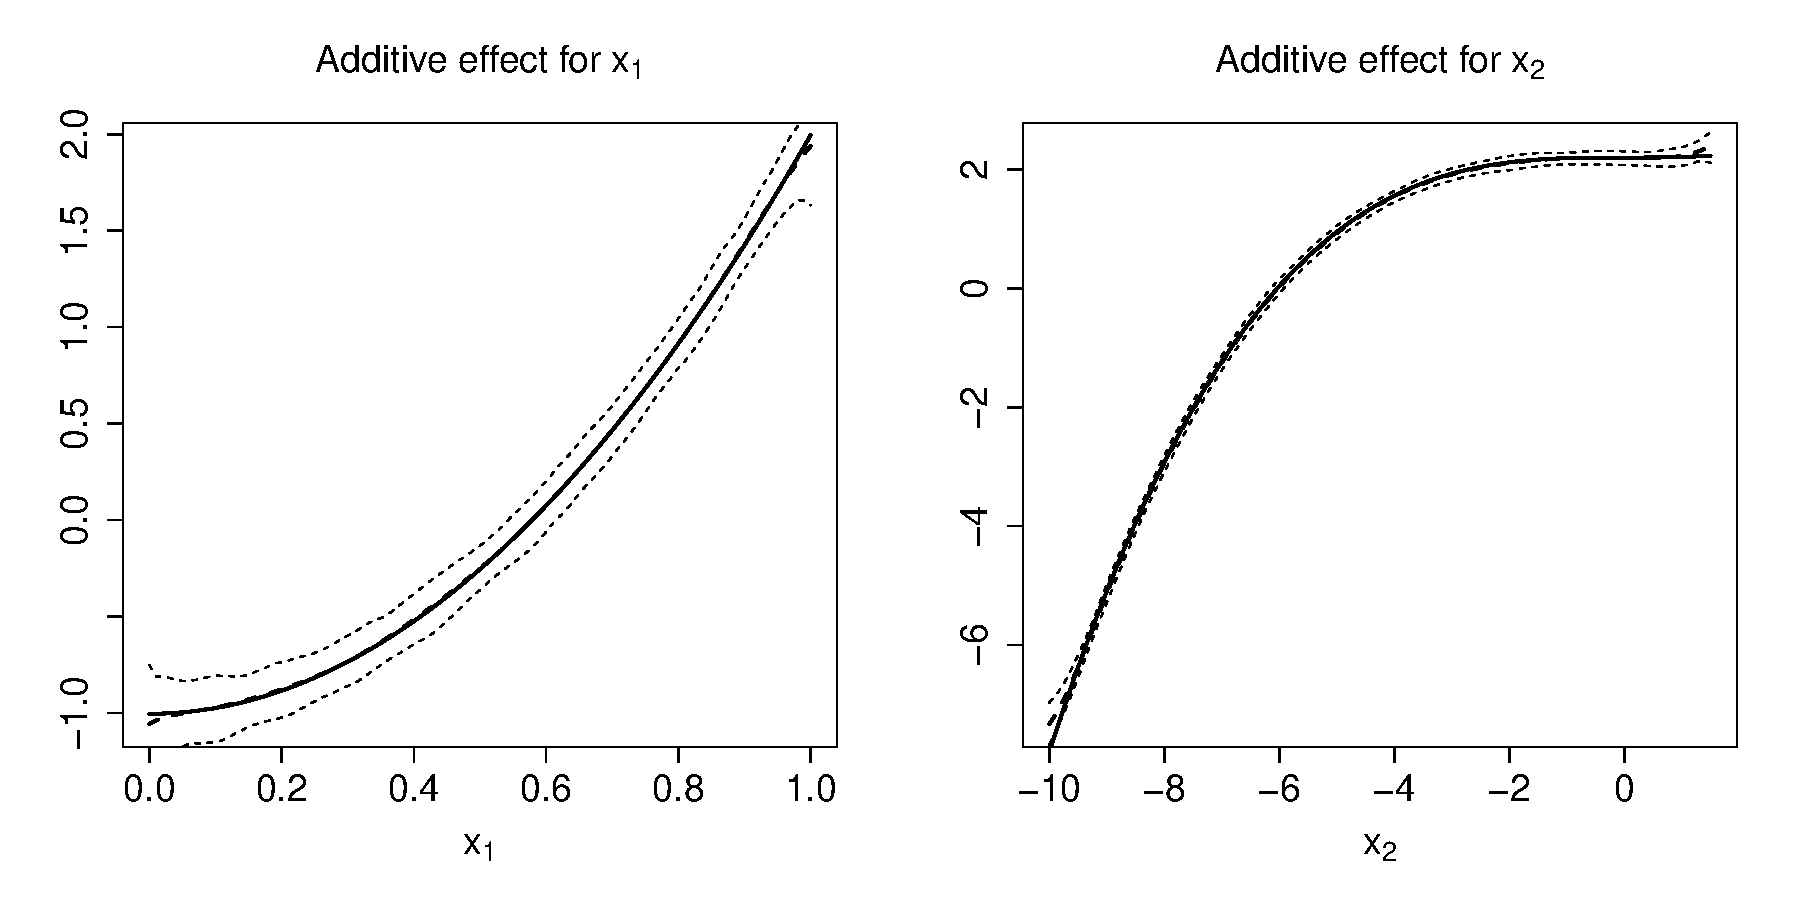
\includegraphics[width=10cm]{additive_gaussian.pdf}}
\subfigure[Bernoulli]{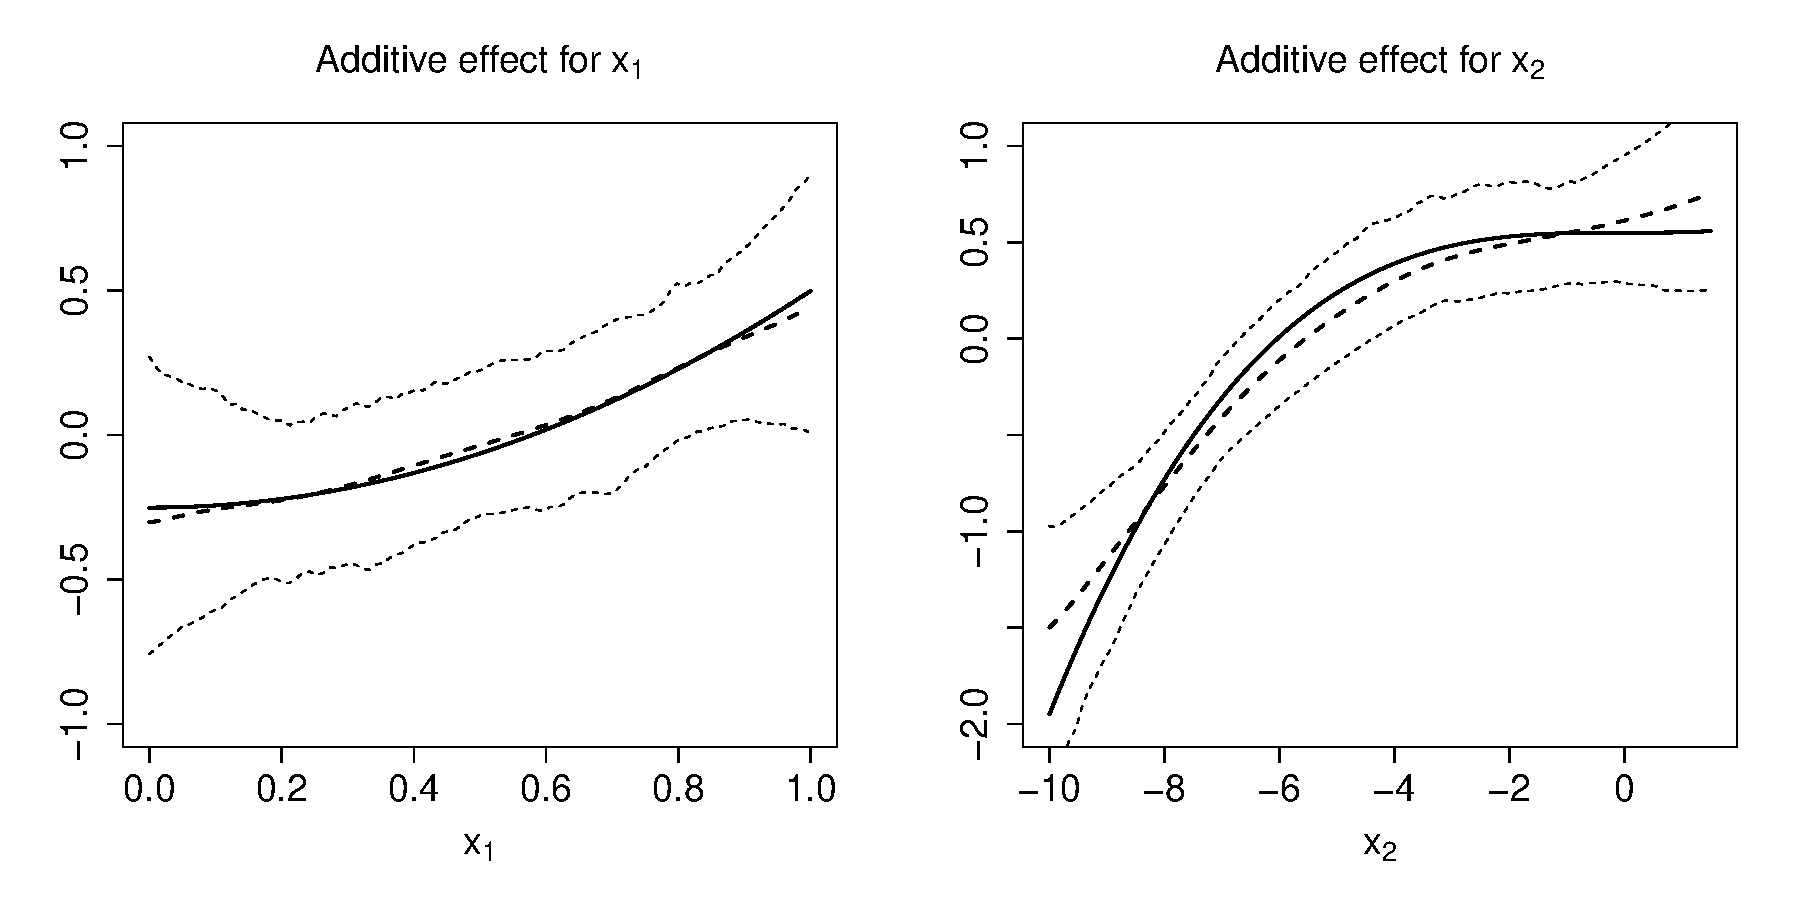
\includegraphics[width=10cm]{additive_binomial.pdf}}  \vspace{-0.25cm}
\caption{The simulation study and Scenario I. From left to right: true curve $g_1$ (solid line) and average estimate $\hat{g}_1$ (dashed line); true curve $g_2$ (solid line) and average estimate $\hat{g}_2$ (dashed line). In both cases, $2.5$ and $97.5$ simulation quantiles are plotted. Top row: Gaussian distribution. Bottom row: Bernoulli distribution. \label{simu-sceI}}
\end{figure}

\begin{figure}[htb]
\centering
\subfigure[Gaussian]{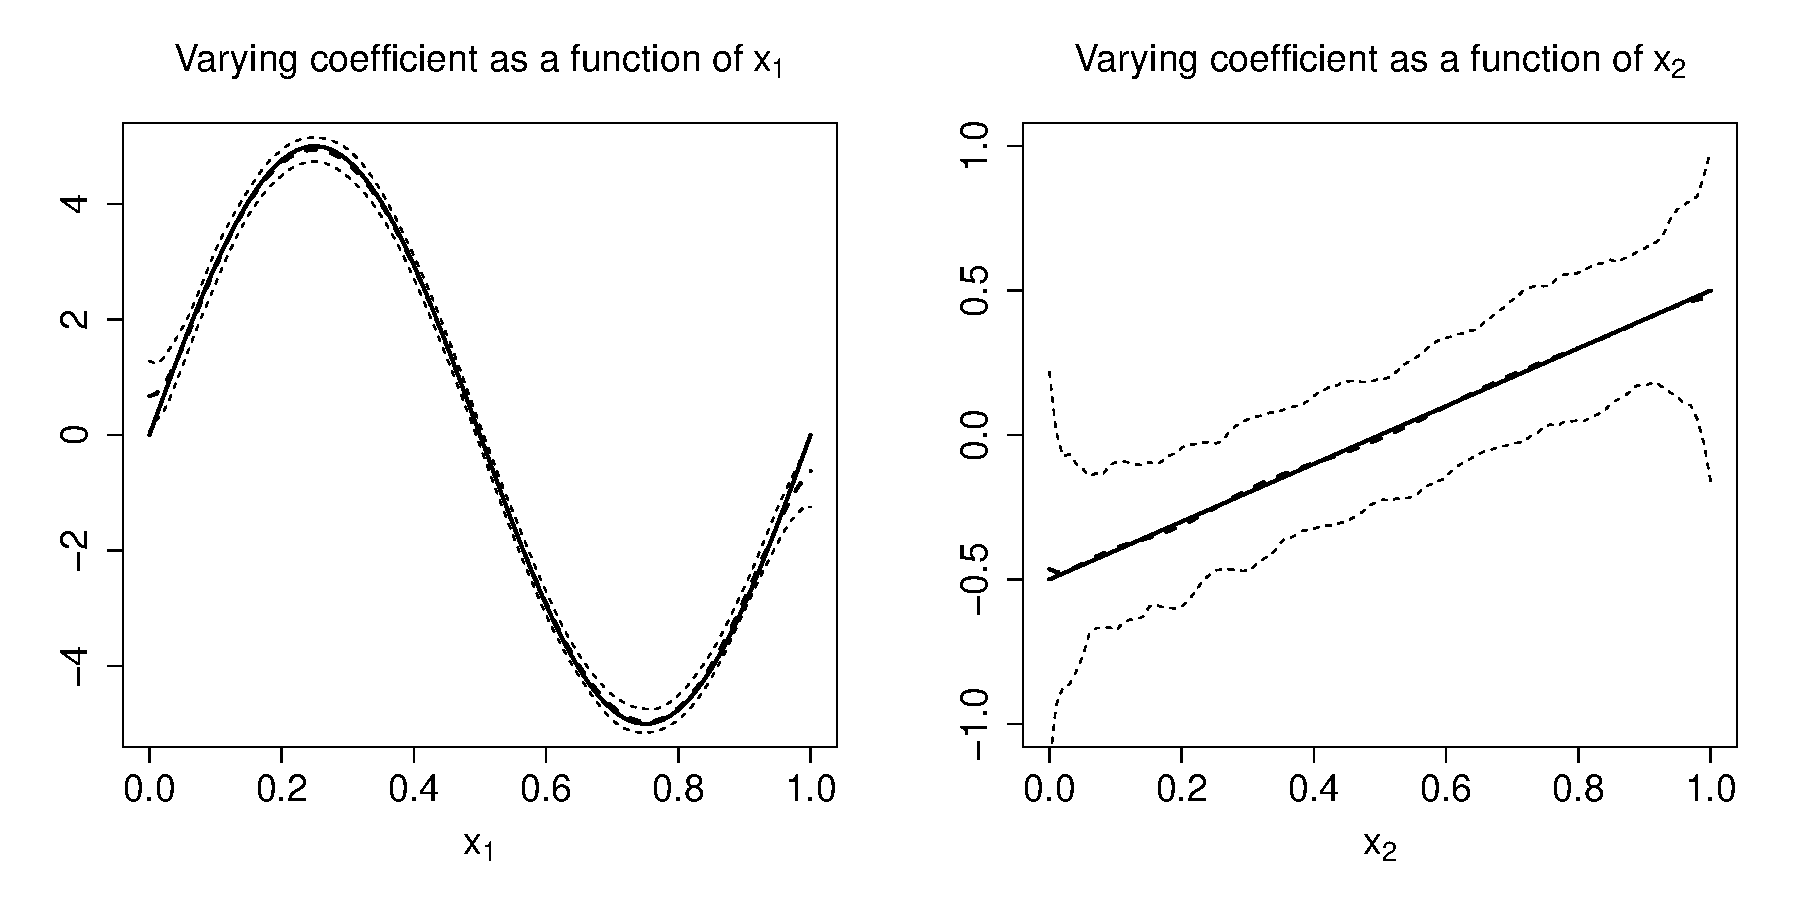
\includegraphics[width=10cm]{vcoeff_gaussian.pdf}}
\subfigure[Bernoulli]{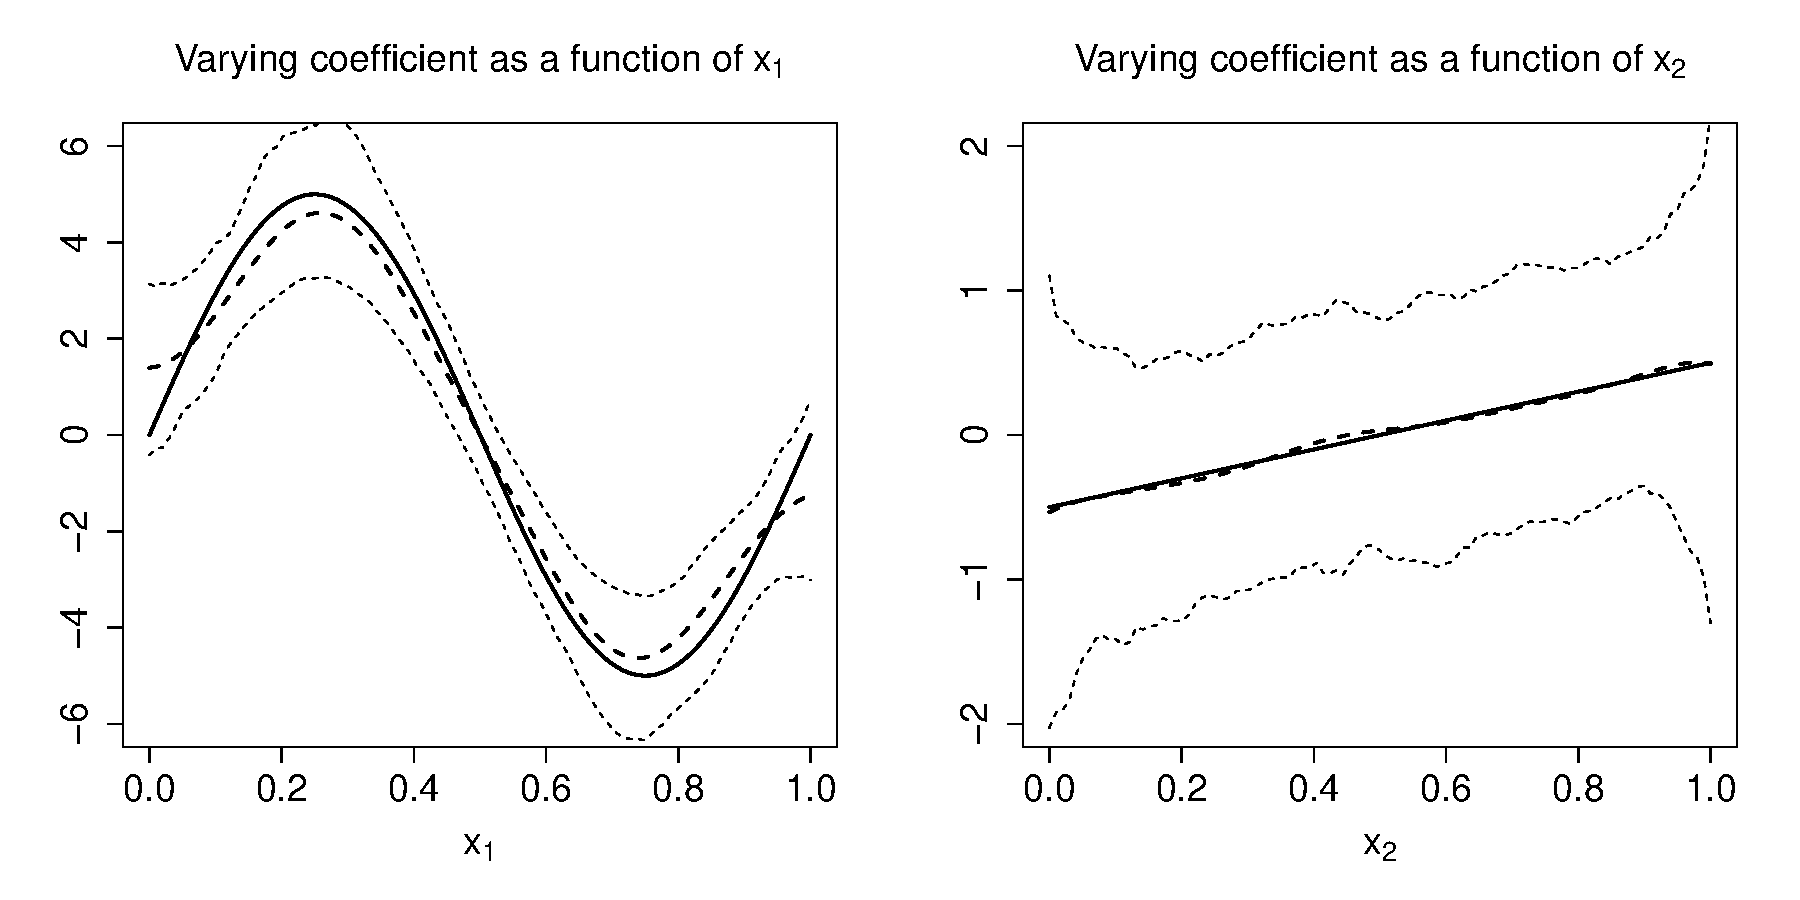
\includegraphics[width=10cm]{vcoeff_binomial.pdf}}
\caption{The simulation study and Scenario II. From left to right: true curve $g_1$ (solid line) and average estimate $\hat{g}_1$ (dashed line); true curve $g_2$ (solid line) and average estimate $\hat{g}_2$ (dashed line). In both cases, $2.5$ and $97.5$ simulation quantiles are plotted. Top row: Gaussian distribution. Bottom row: Bernoulli distribution. \label{simu-sceII}}
\end{figure}

%%%%%%%%%%%%%%%%%%%%%%%%%%%%%%
\section{Examples and applications} \label{sec-examples}
The last section is dedicated to examples with generalized additive and/or varying coefficient, partial linear models with and without heteroscedasticity, given different link functions. In fact, we have examples for each of the three link functions presently available. Among other things, it is shown how the optional weighting can be used to improve efficiency. While some examples are simulated, others illustrate applications from biometrics and health. Finally, we also show how to create useful graphics for interpreting the estimates. 

\subsection{Gaussian simulated data} \label{subsec-gauss}
We start with the presentation of a simulation example for estimating an additive model under heteroscedasticity.
Consider the situation where the variance is a function of a dummy variable, i.e., one faces two noise levels.
This is estimated and afterward used to improve the efficiency of the mean regression. 
As explained in the above sections, this requires a three-step procedure: 
first estimate the mean model, then the variance function, and finally re-estimate the mean model but including the inverse of the variance as an additional weight. 
Consider model
\begin{equation}
Y = \sum_{j=1}^4 g_j(X_j) + \beta \mathbf{1}_{\{X_5 =1\}} + \varepsilon(X_5),\label{ex1}
\end{equation}
with $g_1(x)=2\sin(2x)$, $g_2(x)=x^2$, $g_3(x)=0$, $g_4(x)=x$, $\beta = 1.5$, and $\mathbf{1}_{A}$ denoting the indicator function of event $A$. The covariates $X_1$ to $X_4$ are independent random variables, uniformly distributed on $[-2,2]$, and $X_5 \in Bernoulli (0.4)$. The error term is given by $\epsilon(X_5) \in N(0, \sigma^2 (X_5))$ with  $\sigma(0)=4$ and $\sigma(1)=2$. Data are generated and fitted by
\begin{Schunk}
\begin{Sinput}
R> library(wsbackfit)
R> set.seed(123)
R> # Define the data generating process
R> n <- 1000
R> x1 <- runif(n)*4-2
R> x2 <- runif(n)*4-2
R> x3 <- runif(n)*4-2
R> x4 <- runif(n)*4-2
R> x5 <- as.numeric(runif(n)>0.6)

R> g1 <- 2*sin(2*x1)
R> g2 <- x2^2
R> g3 <- 0
R> g4 <- x4

R> mu <- g1 + g2 + g3 + g4 + 1.5*x5
R> err <- (0.5 + 0.5*x5)*rnorm(n)
R> y <- mu + err

R>  df_gauss <- data.frame(x1 = x1, x2 = x2, x3 = x3, x4 = x4, x5 = as.factor(x5), y = y)

R> # Fit the model with a fixed bandwidth for each covariate
R> m0 <- sback(formula = y ~ x5 + sb(x1, h = 0.1) + sb(x2, h = 0.1) +
+    sb(x3, h = 0.1) + sb(x4, h = 0.1), kbin = 30, data = df_gauss)
\end{Sinput}
\end{Schunk}

A numerical summary of the fitted model can be obtained by calling  \code{print.sback()} or  \code{summary.sback()}
with shortcuts  \code{print()} and  \code{summary()}.

\begin{Schunk}
\begin{Sinput}
R> summary(m0)
\end{Sinput}
\begin{Soutput}
Generalized Smooth Backfitting/wsbackfit:

Call: sback(formula = y ~ x5 + sb(x1, h = 0.1) + sb(x2, h = 0.1) + 
    sb(x3, h = 0.1) + sb(x4, h = 0.1), data = df_gauss, kbin = 30)

Sample size: 1000 

Bandwidths used in model:
 Effect          h  
 sb(x1, h = 0.1) 0.1
 sb(x2, h = 0.1) 0.1
 sb(x3, h = 0.1) 0.1
 sb(x4, h = 0.1) 0.1

Linear/Parametric components:
   Intercept           x1           x2           x3           x4          x51 
 1.342678178  0.346506090 -0.040989607 -0.005250654  1.010634908  1.327833794  
\end{Soutput}
\end{Schunk}

The output obtained from  \code{summary} (corresponding to the prior  \code{sback} call) includes the bandwidth of each nonparametric function, the parameters of the parametric part (here the intercept and $\beta$), and the linear slopes (i.e., the $\alpha_j$ in (\ref{model-new-id}) in Section \nameref{identification}) of the nonparametric functions $g_j$. Recall (Section \nameref{identification}) that the algorithm decomposes each nonparametric function in a linear and a nonparametric local constant one. For a varying coefficient $g_j$, you also get constant $g_{0j}$.

To complement the numerical results, the \pkg{wsbackfit} package also provides graphical outputs by the use of \code{plot}. In particular, it provides the plots of the estimated nonparametric functions. Figure \ref{fig-simul} shows the figures that appear as a result of the following code. We note that through argument \code{select}, the user can specify the model term to be plotted and use \code{ylim} to indicate the range for the y-axis.
This, however, is optional. Alternatively, the program provides plots that automatically explore the variation of the estimates.

\begin{Schunk}
\begin{Sinput}
R> op <- par(mfrow = c(2,2))
R> plot(m0, select = 1, ylim = c(-2.5,2.5))
R> plot(m0, select = 2, ylim = c(-2.5,2.5))
R> plot(m0, select = 3, ylim = c(-2.5,2.5))
R> plot(m0, select = 4, ylim = c(-2.5,2.5))
R> par(op)
\end{Sinput}
\end{Schunk}

\begin{figure}[htb]
	\vspace{-0.5cm}
\centering 
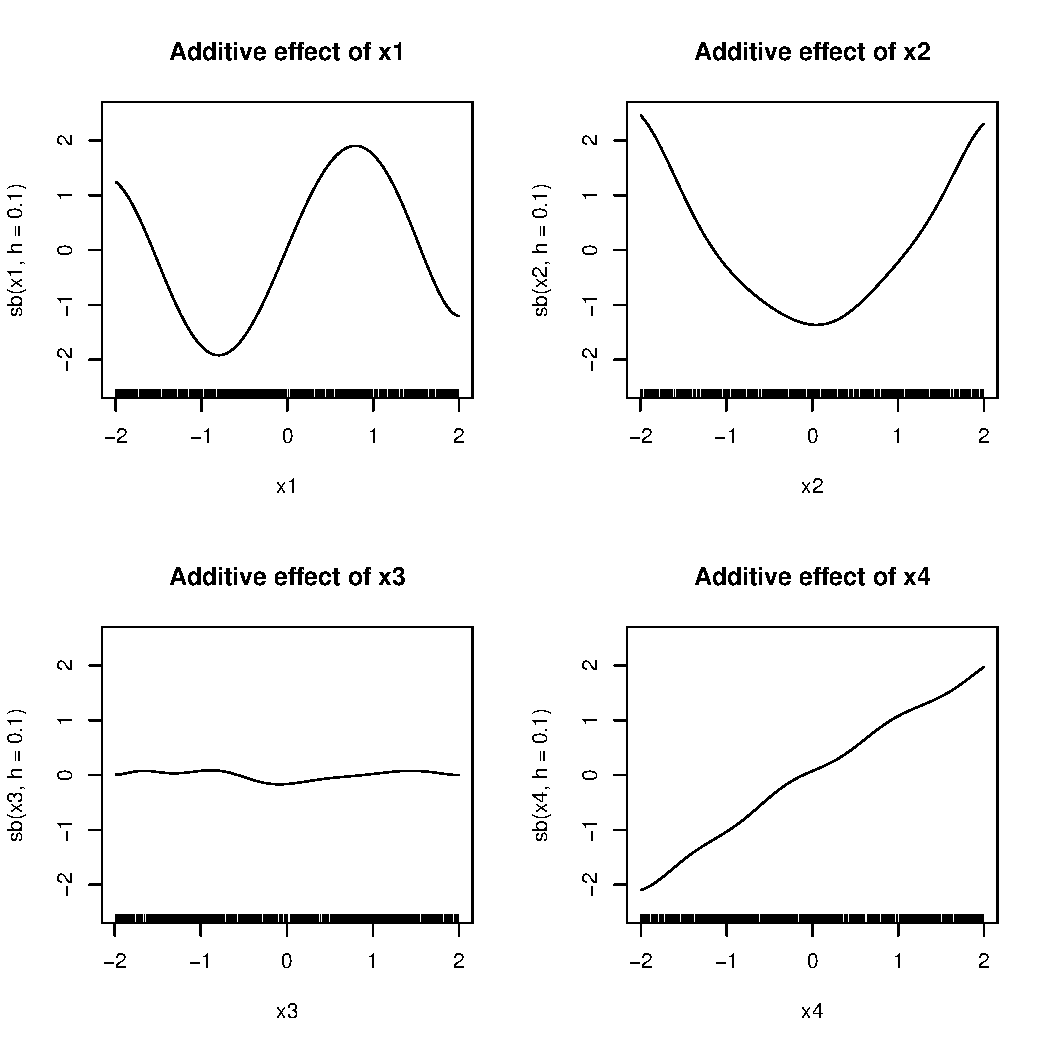
\includegraphics[width=14cm]{Gaussian_Plot_1.pdf} \vspace{-0.75cm}
\caption{Model (\ref{ex1}): Estimated nonparametric functions. These estimates correspond to the sum of the linear and the nonparametric local constant component, recall (\ref{model-new-id}).
\label{fig-simul} }
\end{figure}

If the user is interested in plotting separately each component ($\alpha_j$ and $\tilde g_j$), then the argument  \code{composed} is to be set to  \code{FALSE}. The result is shown in Figure \ref{fig-simul-2}.

\begin{Schunk}
\begin{Sinput}
R> op <- par(mfrow = c(2,2))
R> plot(m0, select = 1, composed = FALSE, ylim = c(-2.5,2.5))
R> plot(m0, select = 2, composed = FALSE, ylim = c(-2.5,2.5))
R> plot(m0, select = 3, composed = FALSE, ylim = c(-2.5,2.5))
R> plot(m0, select = 4, composed = FALSE, ylim = c(-2.5,2.5))
R> par(op)
\end{Sinput}
\end{Schunk}

\begin{figure}[htb]
	 \vspace{-0.5cm}
\centering 
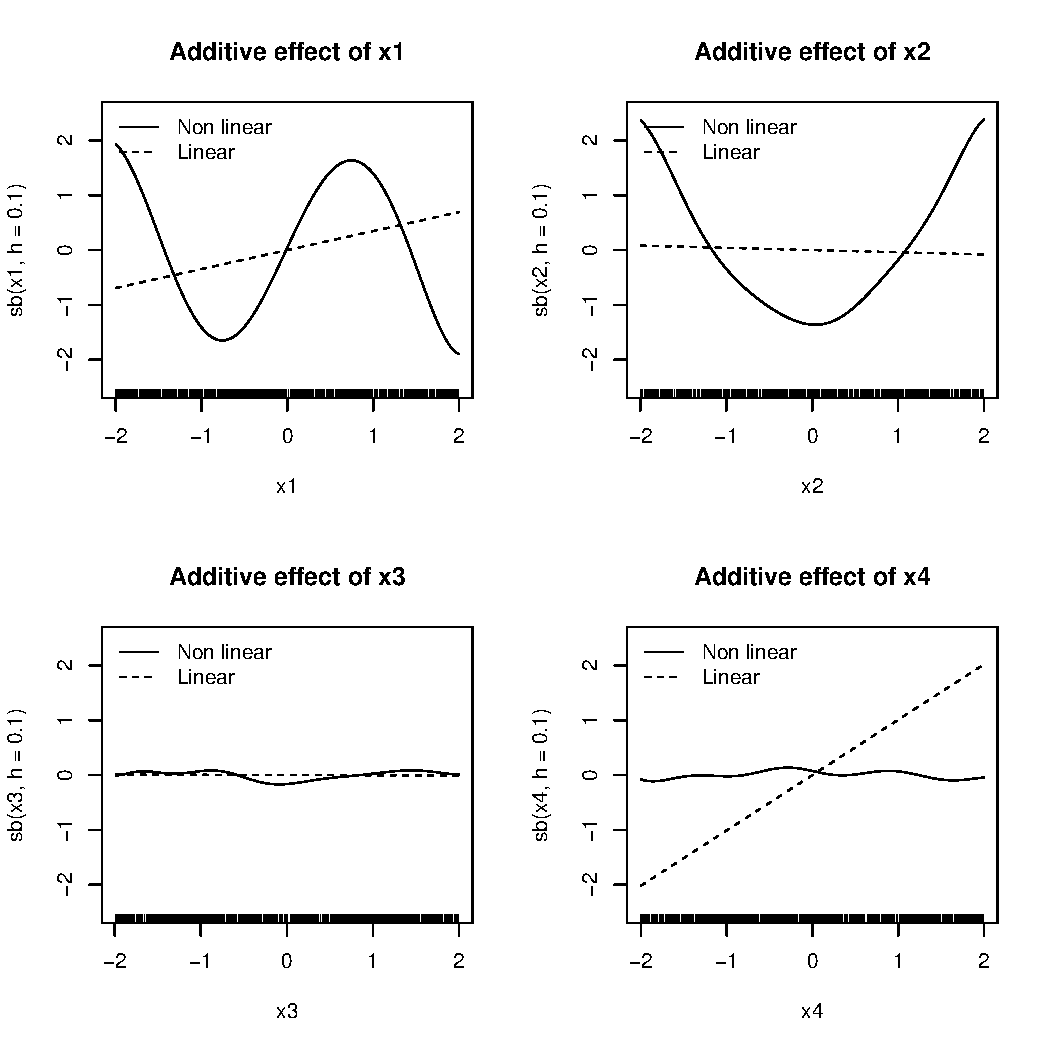
\includegraphics[width=14cm]{Gaussian_Plot_2.pdf}   \vspace{-0.75cm}
\caption{Model (\ref{ex1}): Estimated linear and nonlinear components in which each nonparametric function is decomposed, recall (\ref{model-new-id}).
\label{fig-simul-2}  }
\end{figure}

Note that both \code{summary} and \code{plot} make use of the information contained in the  \code{m0} object.
\begin{Schunk}
\begin{Sinput}
R> names(m0)
\end{Sinput}
\begin{Soutput}
 [1] "call"          "formula"       "data"          "weights"      
 [5] "offset"        "kernel"        "kbin"          "family"       
 [9] "effects"       "fitted.values" "residuals"     "h"            
[13] "coeff"         "err.CV"
\end{Soutput}
\end{Schunk}
This is the list of outputs created by \code{sback}.
A detailed description of what each component of this list contains was given in Table \ref{out_sb}. 
The user can access this information explicitly and individually, may it be to create its own plots or for further reporting.


%In Figure \ref{fig-simul} are plotted the four estimated nonparametric additive functions, together with the true ones, i.e. the underlying data generating functions.
As a next step in the analyses of our example, we use the fitted model to estimate the variance. In our example, this is considered to be a function of the binary covariate $X_5$.
Call

\begin{Schunk}
\begin{Sinput}
R> resid <- y - m0$fitted.values  
R> sig0 <- var(resid[x5 == 0])
R> sig1 <- var(resid[x5 == 1])
\end{Sinput} 
%$
\end{Schunk}

The third and final step is to re-estimate the mean model for efficiency reasons with weights that are the inverse of the estimated variance. The code, including the summary, is

\begin{Schunk}
\begin{Sinput}
R>  w <- x5/sig1 + (1-x5)/sig0
R>  m1 <- sback(formula = y ~ x5 + sb(x1, h = 0.1) + sb(x2, h = 0.1) +  
+ 	sb(x3, h = 0.1) + sb(x4, h = 0.1), 
+	weights = w, kbin = 30, data = df_gauss)
R> summary(m1)
\end{Sinput}
\begin{Soutput}
Generalized Smooth Backfitting/wsbackfit:

Call: sback(formula = y ~ x5 + sb(x1, h = 0.1) + sb(x2, h = 0.1) + 
    sb(x3, h = 0.1) + sb(x4, h = 0.1), data = df_gauss, weights = w, 
    kbin = 30)

Sample size: 1000 

Bandwidths used in model:
 Effect          h  
 sb(x1, h = 0.1) 0.1
 sb(x2, h = 0.1) 0.1
 sb(x3, h = 0.1) 0.1
 sb(x4, h = 0.1) 0.1

Linear/Parametric components:
  Intercept          x1          x2          x3          x4         x51 
 1.31707760  0.32888538 -0.01262394  0.01222234  1.00289877  1.33368035 
\end{Soutput}
\end{Schunk}


In the previous fits of this example, we specified all bandwidths used. For the rest of this example, let us consider the case when we ask the program to choose the bandwidths via k-fold CV. We do this for all nonparametric functions, using the following code in which, for the sake of clarity and presentation, we specify \code{h = -1} although this is actually the default.
For convenience, we also call the \code{summary} command directly:

\begin{Schunk}
\begin{Sinput}
R> m1cv <- sback(formula = y ~ x5 + sb(x1, h = -1) + sb(x2, h = -1) + 
+   sb(x3, h = -1) + sb(x4, h = -1), weights = w, kbin = 30,  
+   bw.grid = seq(0.01, 0.99, length = 30), KfoldCV = 5, data = df_gauss)
R> summary(m1cv)
\end{Sinput}

\begin{Soutput}
Generalized Smooth Backfitting/wsbackfit:

Call: sback(formula = y ~ x5 + sb(x1, h = -1) + sb(x2, h = -1) + sb(x3, 
    h = -1) + sb(x4, h = -1), data = df_gauss, weights = w, bw.grid = seq(0.01, 
    0.99, length = 30), KfoldCV = 5, kbin = 30)

Sample size: 1000 

Bandwidths used in model:
 Effect             h     
 sb(x1, h = 0.0892) 0.0892
 sb(x2, h = 0.0887) 0.0887
 sb(x3, h = 0.0907) 0.0907
 sb(x4, h = 0.0912) 0.0912

Linear/Parametric components:
  Intercept          x1          x2          x3          x4         x51 
 1.31708207  0.32881191 -0.01219359  0.01247328  1.00258427  1.33366258 
\end{Soutput}
\end{Schunk}

We do not further discuss the results because their interpretation is the same as before, also because the automatically found data-driven optimal bandwidths are close to what we used as prefixed bandwidths in the former codes. We conclude this section with a brief example in which we specify the bandwidths for some of the nonparametric functions, while for the remaining ones, we let our CV procedure select the bandwidths. For brevity, we skip output and discussion.

\begin{Schunk}
\begin{Sinput}
R> m2cv <- sback(formula = y ~ x5 + sb(x1, h = 0.1) + sb(x2, h = -1) + 
+ 	sb(x3, h = 0.1) + sb(x4, h = 0.1), 
+	weights = w, kbin = 30, KfoldCV = 5, data = df_gauss)
\end{Sinput}
\end{Schunk}



\subsection{Post-operative infection data}

The next example is an application with data studied, among others, in \citet{RS2010}. 
They were taken from a prospective analysis conducted at the University Hospital of Santiago de Compostela in the North of Spain. A total of $n=2318$ patients who underwent surgery at this center between January 1996 and March 1997 were considered. 
The main interest is learning about indicators that could predict whether patients may suffer (\code{inf=1}) or not post-operative infection (\code{inf=0}), and to see how they relate to the risk of infection. 
Such predictive indicators could be various, but given the previous studies we concentrate on the pre-operative values of plasma glucose (\code{gluc}) concentration (measured in mg/dl), and lymphocytes (\code{linf}, expressed as relative counts (in \% of the white blood cell count). The data can be found in \pkg{wsbackfit} under the name \code{infect}. 

\begin{Schunk}
\begin{Sinput}
R> data(infect)
R> head(infect)
\end{Sinput}
\begin{Soutput}
 age sex linf gluc diab inf
1  85   2   28   55    2   0
2  38   1   18   56    2   1
3  49   2   29   56    2   1
4  63   2   20   60    2   0
5  91   2   17   62    2   0
6  26   2   22   66    2   0
\end{Soutput}
\end{Schunk}

In the original studies, it was controlled for other covariates like  \code{age} (in years) and  \code{sex} (coded as 1 = male; 0 = female). For illustrative purposes, we limit our analysis to the investigation of the association of the risk of post-operative infections  \code{inf} with the predictors  \code{linf} and  \code{gluc}, putting all other covariates aside. It is well known that the effect of  \code{linf} on  \code{inf} varies strongly with the 
concentration of  \code{gluc}. Therefore, one may think of a generalized varying coefficient model of type
\begin{align}
& \log \frac{P\left(\mbox{inf} = 1 \vert \mbox{linf},\mbox{gluc} \right)}{1-P\left( \mbox{inf} = 1 \vert
\mbox{linf}, \mbox{gluc} \right)}  = g_0 + g_1(\mbox{gluc}) + g_2 (\mbox{gluc})\mbox{linf} \nonumber \\
& = g_0 + \left(\alpha_{1} \cdot \mbox{gluc} + \tilde{g}_1(\mbox{gluc})\right) + \left(g_{20} + \alpha_{2} \cdot \mbox{gluc} + \tilde{g}_2(\mbox{gluc})\right)\mbox{linf}, \label{ipo2}
\end{align}
in which we are working with the Logit link. This can be fitted using of the following code

\begin{Schunk}
\begin{Sinput}
R> data(infect)
R> # Generalized varying coefficient model with binary response
R> m2 <- sback(formula = inf ~ sb(gluc, h = 10) + sb(gluc, by = linf, h = 10), 
+   data = infect, kbin = 15, family = "binomial")
 
R> summary(m2)
\end{Sinput}
\begin{Soutput}
Generalized Smooth Backfitting/wsbackfit:

Call: sback(formula = inf ~ sb(gluc, h = 10) + sb(gluc, by = linf, 
    h = 10), data = infect, kbin = 15, family = "binomial")

Sample size: 2312 

Bandwidths used in model:
 Effect                      h 
 sb(gluc, h = 10)            10
 sb(gluc, by = linf, h = 10) 10

Linear/Parametric components:
    Intercept          gluc          linf     gluc:linf 
-1.4155401353  0.0068313875 -0.0346648080 -0.0000456441  
\end{Soutput}
\end{Schunk}

Note that this model, recall \eqref{ipo2}, contains, in addition to the constant term (intercept), 
the main linear effects of \code{gluc} $\alpha_1$ and  \code{linf} $g_{20}$, and the linear interaction between  \code{gluc} and  \code{linf} $\alpha_2$, all provided in the very last line. Our bandwidths have been chosen for graphical convenience. The graphical output, i.e., the plots of the estimated nonparametric functions, is obtained by the code

\begin{Schunk}
\begin{Sinput}
R> op <- par(mfrow = c(1,3))
R> plot(m2, composed = FALSE, ask = FALSE, cex.main = 2, cex = 2, cex.lab = 1.5, 
+    cex.axis = 2)
R> par(op)

R> op <- par(mfrow = c(1,3))
R> plot(m2, composed = FALSE, ask = FALSE, cex.main = 2, cex = 2, cex.lab = 1.5, 
+    cex.axis = 2)
R> par(op)
\end{Sinput}
\end{Schunk}

\begin{figure}[htb]
\centering
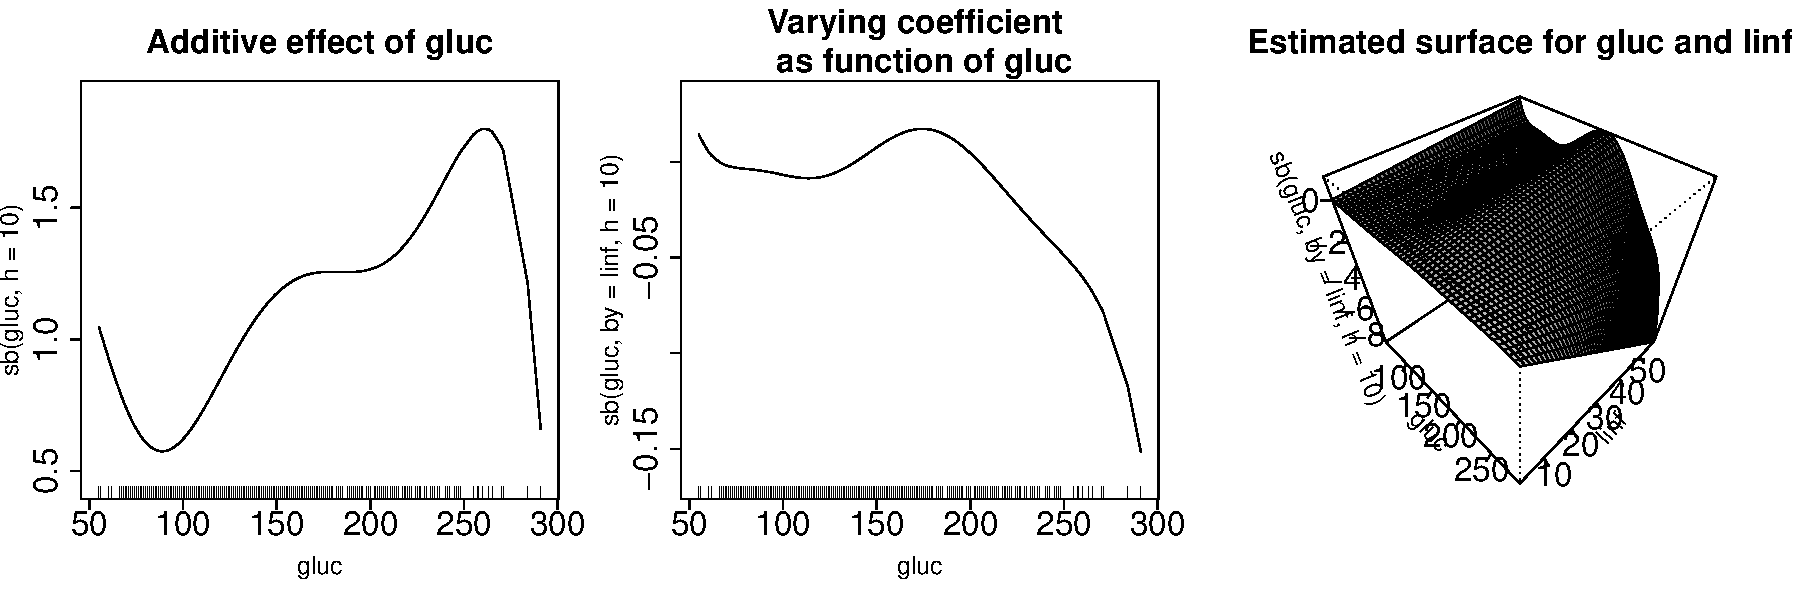
\includegraphics[width=1\textwidth]{Infec_Plot_1.pdf}
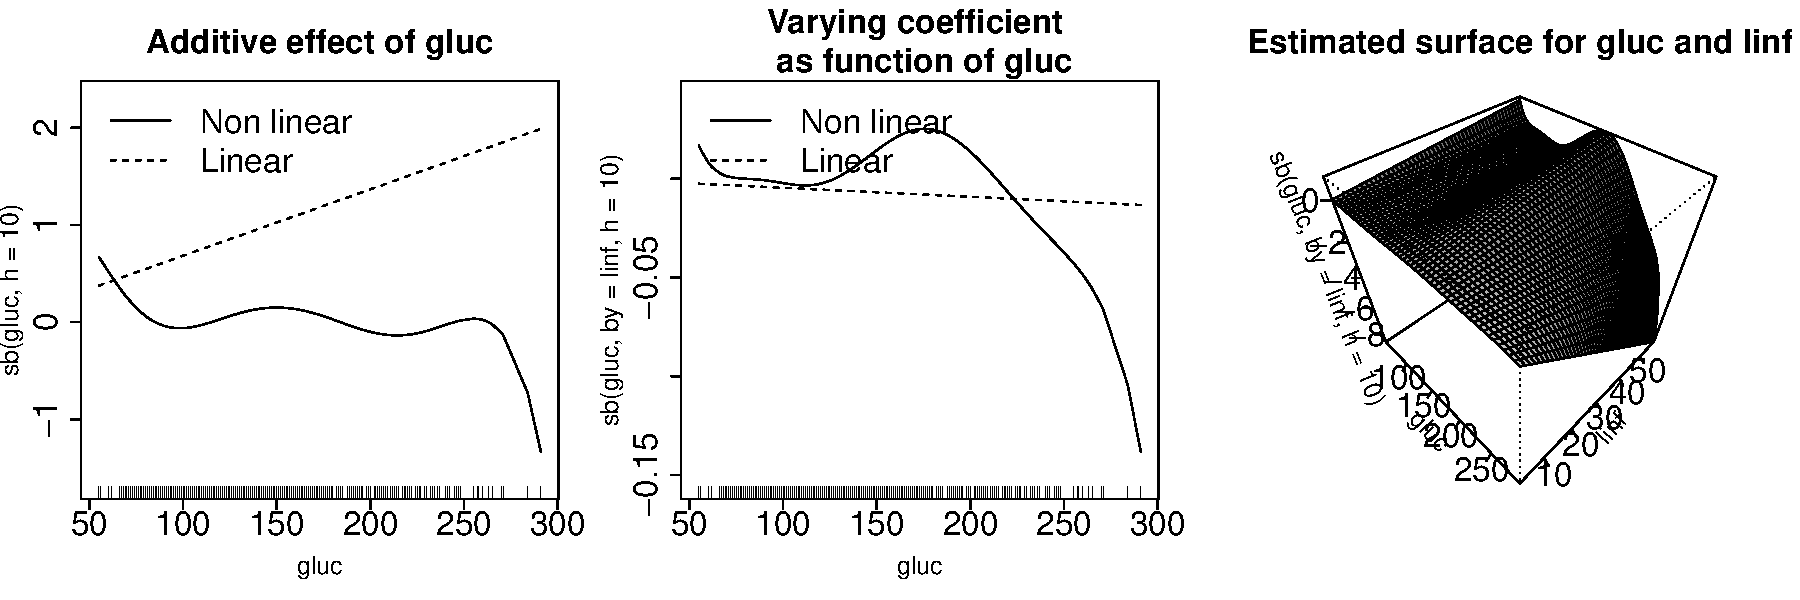
\includegraphics[width=1\textwidth]{Infec_Plot_2.pdf}
\caption{Post-operative infection data. Upper row: estimates of $\alpha_{1} \cdot gluc + \tilde{g}_1(gluc)$ (left), $\alpha_{2} \cdot gluc + \tilde{g}_2(gluc)$ (middle), and $\left(\alpha_{2} \cdot gluc + \tilde{g}_2(gluc)\right)linf$ (right) obtained from model (\ref{ipo2}). The plots on the left and the center in the bottom line show the estimates of the linear and nonlinear components separately. In this example, the right plot is simply repeated.\label{fig-ipo}}
\end{figure}

In Figure \ref{fig-ipo}, you see the functionals of the nonparametric additive effect of  \code{gluc} on the index $\eta$
(left column), the varying coefficient (center), and the interaction surface (right column), because the interest is in revealing how the effect of lymphocytes changes with the plasma glucose concentration. If the interest is also in knowing the resulting probabilities of post-operational infection, then there are the options of plotting the two-dimensional function as a (dynamic) 3-D plot (less appropriate for printed figures) or by contour plots as done in Figure \ref{fig-ipo2}. This was created with the code  

\begin{Schunk}
\begin{Sinput}
R> # Dataframe for prediction (and plotting)
R> ngrid <- 30
R> gluc0 <- seq(50,190, length.out=ngrid)
R> linf0 <- seq(0,45, length.out=ngrid)
R> infect_pred  <- expand.grid(gluc = gluc0, linf = linf0)
 
R> m2p <- predict(m2, newdata = infect_pred)
R> n <- sqrt(nrow(infect_pred))
R> Z <- matrix(m2p$pfitted.values, n, n)
R > filled.contour(z = Z, x = gluc0, y = linf0,
+ xlab = "Glucose (mg/dl)", ylab = "Lymphocytes (%)", 
+ col = cm.colors(21))
\end{Sinput}
\end{Schunk}
 
\begin{figure}[htb]
\centering
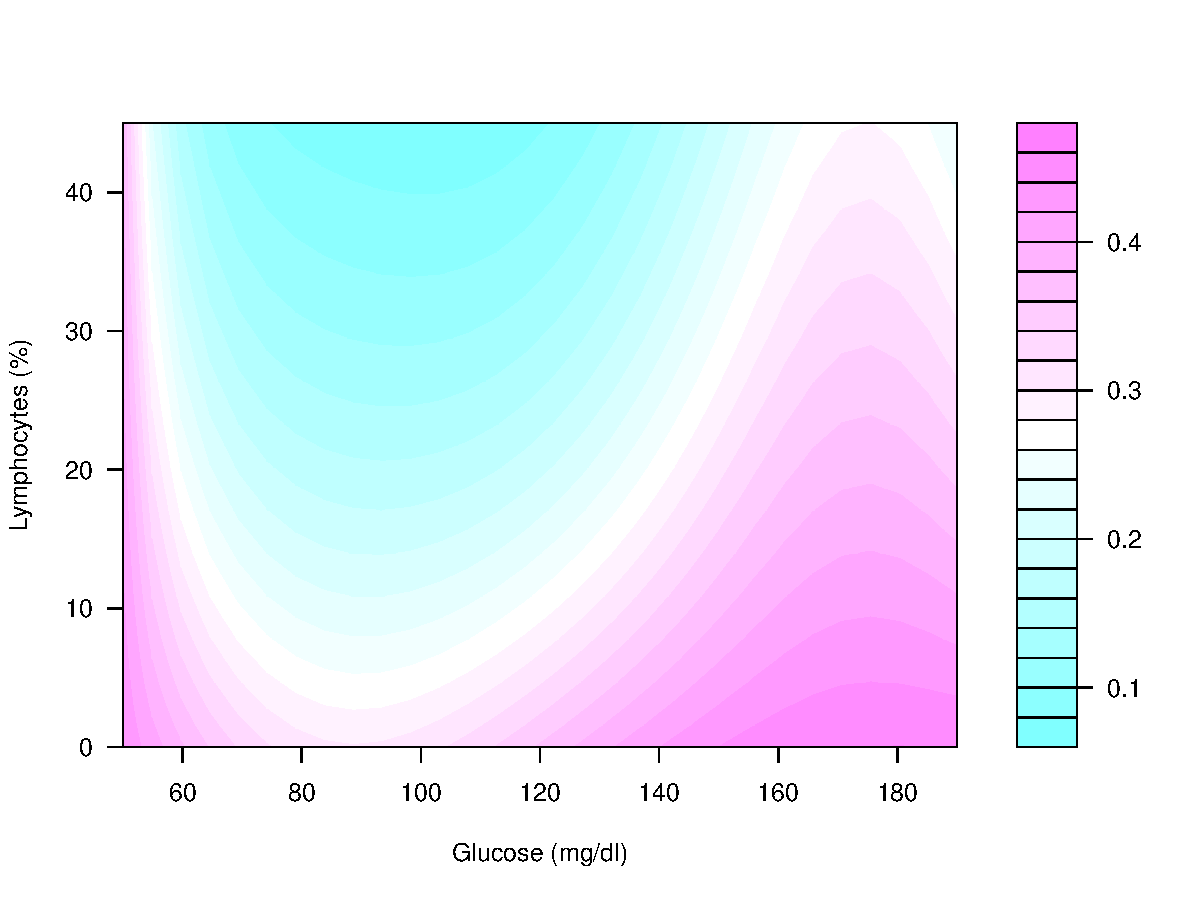
\includegraphics[width=11cm]{Infec_Plot_3.pdf}  \vspace{-0.5cm}
\caption{The post-operative infection data: Estimated probability of post-operational infection.  \label{fig-ipo2} }
\end{figure}

As can be seen from Figure \ref{fig-ipo2}, high levels of  \code{gluc} increase the post-operative infection risk, but higher  \code{linf} values can mitigate this effect significantly.  



\subsection{Poisson regression with offset}\label{subsec-PoissExample}

Let us now consider a simulated example that illustrates the use of Poisson regression with a nontrivial use of option  \code{offset}.
We simulate data where each subject may have different levels of exposure to the event of interest.
As explained in the above sections, this can be handled with the  \code{offset} option. More specifically, for the level of exposure $P$ we consider 
\[
Y\in Poisson \left( { P \cdot \exp \left({ 2+ 3X_1^2+5X_2^3 }\right) }\right) \ .
\]
In our simulations, $X_1$ and $X_2$ were generated as independent continuous random variables uniformly distributed on $[-1,1]$, and $P$ as an approximately uniformly distributed discrete variable with support $\{50,51,\ldots ,100\}$.
The complete code for simulation, estimation, and summary of results is 

\begin{Schunk}
\begin{Sinput}
R> set.seed(123)
R> # Generate the data
R> n <- 1000
R> x1 <- runif(n,-1,1)
R> x2 <- runif(n,-1,1)
R> eta <- 2 + 3*x1^2 + 5*x2^3
R> exposure <- round(runif(n, 50, 500))
R> y <- rpois(n, exposure*exp(eta))
R> df_poiss <- data.frame(y = y, x1 = x1, x2 = x2)
R> # Fit the model
R> m4 <- sback(formula = y ~ sb(x1, h = 0.1) + sb(x2, h = 0.1), 
+	data = df_poiss, offset = log(exposure), 
+	kbin = 30, family = "poisson")

R> summary(m4)
\end{Sinput}
\begin{Soutput}
Generalized Smooth Backfitting/wsbackfit:

Call: sback(formula = y ~ sb(x1, h = 0.1) + sb(x2, h = 0.1), data = df_poiss, 
    offset = log(exposure), kbin = 30, family = "poisson")

Sample size: 1000 

Bandwidths used in model:
 Effect          h  
 sb(x1, h = 0.1) 0.1
 sb(x2, h = 0.1) 0.1

Linear/Parametric components:
 Intercept         x1         x2 
3.00099626 0.09698672 3.06092318
\end{Soutput}
\end{Schunk}

As for the previous examples, a graphical output can be obtained using the  \code{plot} function like in the following code. The results are shown in Figure \ref{fig-simul-3}, namely the additive components.

\begin{Schunk}
\begin{Sinput}
R> op <- par(mfrow = c(1,2))
R> plot(m4, ask = FALSE)
R> par(op)
\end{Sinput}
\end{Schunk}

\begin{figure}[htb]
\vspace{-0.25cm} 
\centering 
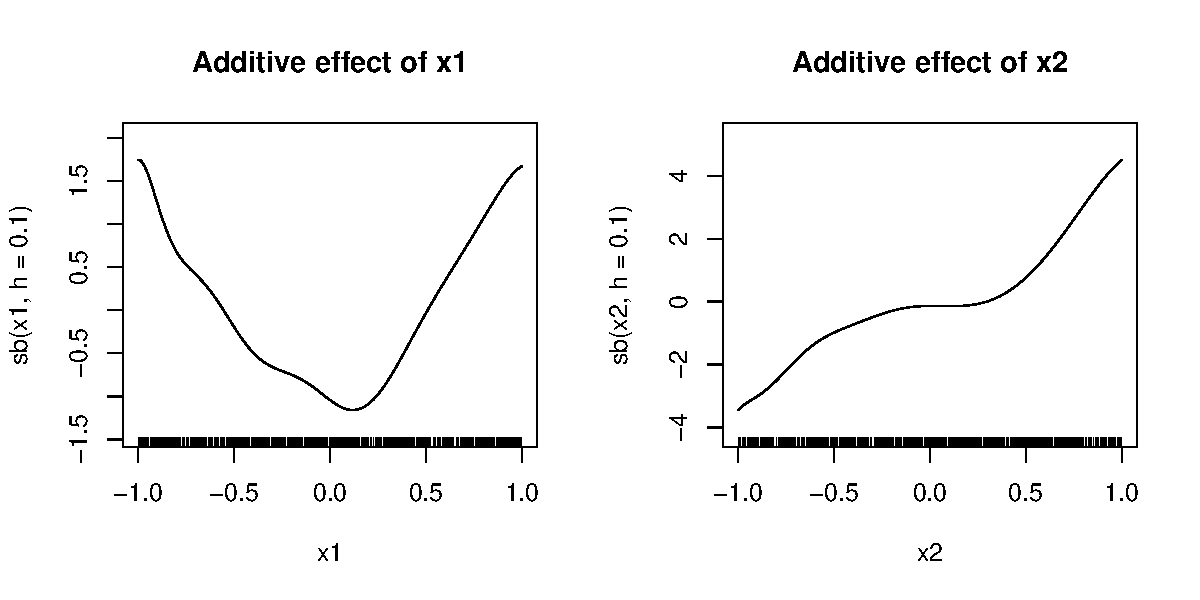
\includegraphics[width=14cm]{Poisson_Plot.pdf}  
\vspace{-0.9cm}
\caption{The Poisson Simulated Data: Estimated nonparametric functions. %with data generating functions.} 
\label{fig-simul-3} }
\end{figure}



\section{Summary}\label{sec-conclusions}

We have first given a general introduction into the class of Generalized Structures Models, together with the powerful kernel-based smooth backfitting estimator to fit the members of this model class. This was accompanied by a (certainly incomplete) literature review and closed
with a small review and discussion of existing methods and software for similar and related models.
Except for the varying coefficient model estimator in the \pkg{np} package, they are all based on splines. We concluded that, while there is a huge body of literature on SB and its advantages, it is hardly used in practice due to the lack of software. The \pkg{wsbackfit} package intends to close this gap.

Next, we provided some insight into the weighted SB and the objective function that is minimized by our algorithm. This allowed us to better explain the users' options like  \code{weights} and  \code{offset}. We outlined which models can be estimated by the presently available package. The description of the procedure was complemented by a section on the implemented CV, bandwidth choice, binning, convergence, and identification issues to clarify the location and scaling of the resulting estimates. 

The package description has been kept condense but its use has been illustrated along several examples that cover some of the estimable models. They comprise the use of all options provided. Moreover, the numerical examples give an idea of the estimators' performance. For more details, we recommend consulting the cited articles dealing with the particular models.

We believe that this package is an important enrichment of the existing methods with many useful applications of flexible data analysis and prediction.   
It can almost straightforwardly be used for testing 
\citep{CadarsoEtal2006,MammenSperlich2021} or
studying  the heterogeneity of causal effects
\citep{BeniniSperlich2021}
and many other interesting applications.
The next challenge will be the extension of this package to cover the analysis of more complex data \citep{JeonPark2020}.
The package is not just open for extensions. We explicitly invite people to contribute.

\bibliography{roca-rodriguez-sperlich}

\address{Javier Roca-Pardi\~{n}as \\
	Department of Statistics and O.R.\\
	University of Vigo, Spain.\\
	E-mail: \email{roca@uvigo.es}}
	
\address{Mar\'ia Xos\'e Rodr\'iguez-\'Alvarez\\
	BCAM - Basque Center for Applied Mathematics\\
	\emph{and}\\
	IKERBASQUE, Basque Foundation for Science\\
	Alameda de Mazarredo, 14\\
	E-48009 Bilbao, Basque Country, Spain\\
	E-mail: \email{mxrodriguez@bcamath.org}}
	
\address{Stefan Sperlich\\
	Geneva School of Economics and Management\\
	University of Geneva\\
	Bd du Pont d'Arve 40, CH - 1211 Gene\`{e}ve 4, Switzerland\\ 
	E-mail: \email{Stefan.Sperlich@unige.ch}}


